\documentclass[a4paper]{sig-alternate-05-2015}

%% regra para substituir as aspas convencionais para o padrão do latex :)
%% https://tex.stackexchange.com/questions/10670/quotes-in-latex
\newif\ifquoteopen
\catcode`\"=\active % lets you define `"` as a macro
\DeclareRobustCommand*{"}{%
	\ifquoteopen
	\quoteopenfalse ''%
	\else
	\quoteopentrue ``%
	\fi
}

% Deactive with: \catcode`\"=12\relax % changes `"` back to normal
\renewcommand{\rmdefault}{phv} % Arial
\renewcommand{\sfdefault}{phv} % Arial

\usepackage{ae}
\usepackage{aecompl}
\usepackage{algorithm2e}
\usepackage{blindtext}
\usepackage{booktabs}
\usepackage{caption}
\usepackage{color}
\usepackage{etoolbox}
\usepackage{float}
\usepackage{framed}
\usepackage{graphicx}
\usepackage{hyphenat}
\usepackage{hyperref}
\usepackage{listings}
\usepackage{makecell}
\usepackage{pslatex}
\usepackage[portuguese]{babel}
\usepackage{ragged2e}
\usepackage[T1]{fontenc}
\usepackage{tabularx}
\usepackage{upquote}
\usepackage[utf8]{inputenc}
\usepackage{xcolor}

% add sintax highlight to qml code
\lstdefinelanguage{qml} {
	morekeywords={Item, property, Component, Components, onCompleted, var, Connections, target, onEventNotify, if, else, RequestHttp, import, baseUrl, basicAuthorizationUser, basicAuthorizationPassword, onError, Database, id, jsonColumns, tableName, pkColumn, onItemLoaded, text, Label, Image, Column, spacing},
	keywordstyle=\color{red},
	showstringspaces=true,
	basicstyle=\small,
	morestring=[b]",
	commentstyle=\color{blue},
	frame=trBL,
	%numbers=left,
	%numberstyle=\tiny,
	%stepnumber=1,
	tabsize=4,
}

% adiciona o prefixo dos exemplos de código QML para "Algoritmo"
\renewcommand{\lstlistingname}{Algoritmo}

\graphicspath{{images/}}
\hyphenation{mate-mática recu-perar}

\begin{document}
	\makeatletter
	\def\fnum@figure{Figura \thefigure}
	\def\fnum@table{Tabela \thetable}
	\makeatother

	\title{Uma Arquitetura de Referência Baseada em Plugins para Sistemas de Informação Mobile}

	\numberofauthors{2}
	\author{
		% 1st. author
		\alignauthor
		Enoque Joseneas\titlenote{Graduando em Análise e Desenvolvimento de Sistemas}\\
		\affaddr{Instituto Federal da Bahia}\\
		\affaddr{Rua Emídio dos Santos, S/N, Barbalho}\\
		\affaddr{Salvador-Ba, Brasil}\\
		\email{enoquejoseneas@ifba.edu.br}
		% 2nd. author
		\alignauthor
		Sandro Andrade\titlenote{Prof. Doutor em Ciência da Computação}\\
		\affaddr{Instituto Federal da Bahia}\\
		\affaddr{Rua Emídio dos Santos, S/N, Barbalho}\\
		\affaddr{Salvador-Ba, Brasil}\\
		\email{sandroandrade@ifba.edu.br}
	}
	\maketitle

	\section*{RESUMO}
	O desenvolvimento de aplicativos móveis trouxe uma série de desafios para a ciência da computação. Com limitações de recursos como a bateria, armazenamento e memória, o desenvolvimento de software para dispositivos móveis impõe requisitos não-funcionais importantes a serem considerados no projeto de aplicativos. Com a popularização da internet e a expansão das redes móveis, os aplicativos tornaram-se popular e projetá-los de forma fácil com componentes de alto nível, baixo acoplamento e bom desempenho não é uma tarefa trivial. Este trabalho apresenta uma arquitetura de referência para o desenvolvimento de aplicativos móveis orientado a plugins no contexto de sistemas de informação, proporcionando baixo acoplamento entre os componentes e escalabilidade de recursos através de plugins, dispondo de componentes genéricos reutilizáveis, além de componentes de alto nível para recursos básicos como requisições HTTP, persistência de dados, notificações ao usuário e comunicação entre objetos através de eventos.

	\keywords{Aplicativos Móveis; Arquitetura de Software; Sistemas de Informação.}

	% sections
	% Outra justificativa:
% A atitude mais comum no desenvolvimento de uma nova aplicação tem sido a escolha de
% um framework de desenvolvimento disponível no mercado e de conhecimento da equipe que
% irá implementá-lo. Nesse ponto é que começam a aparecer os problemas, como forte
% acoplamento tecnológico, desperdício de esforços, dificuldade de gerenciamento de versão,
% uso exagerado e desnecessário de recursos computacionais, problemas estruturais, aumento do
% custo global, dificuldade de adequação a novas tecnologias, latência na geração de novas
% versões, etc. Todos esses problemas, naturais do processo de desenvolvimento de software,
% emperram a fabricação de software nas mais diversas áreas de aplicação.


\section{Introdução}\label{sec:introducao}
%--------------------------%
%Falar sobre a popularização dos dispositivos móveis e da Internet.%
%Falar sobre as mudanças introduzidas pelos dispositivos móveis nas formas de comunicação em sociedade.%
%--------------------------%
Os dispositivos móveis apresentam a cada dia novas oportunidades e desafios para as tecnologias de informação, tais como o acesso ubíquo, a portabilidade, a democratização do acesso à informação além de novas oportunidades de negócio \cite{levy_2002}. Com a expansão da Internet e o grande volume de dados compartilhados nas redes sociais e aplicativos de troca de mensagens, surgiram novos paradigmas (e.g. \textit{Big Data}, \textit{Cloud Computing}, \textit{NoSQL}, etc.), novas tecnologias como o \textit{Push Notification} e também novas oportunidades de trabalho e profissões (e.g. O analista de dados, o desenvolvedor mobile, o \textit{design UX} e etc.), além de pesquisas importantes na ciência da computação que abrange tanto hardware como software.\par

Os smartphones inovam a cada dia diversas áreas do conhecimento, tais como a engenharia elétrica, no projeto de baterias cada vez mais eficientes, o design, no projeto de interfaces cada vez mais intuitivas e influenciam diretamente na evolução da Internet e dos meios de comunicação como as redes móveis que expandem as áreas de cobertura para atender ao crescente número de aparelhos conectados. Os dispositivos móveis também permitem bons empreendimentos através dos aplicativos. Atualmente, o número de downloads cresce a cada dia na \textit{App Store} e \textit{Google Play}, demonstrando uma certa disponibilidade dos usuários de passarem cada vez mais tempo utilizando os aplicativos do que os próprios navegadores de Internet \cite{D&T}. Através dos aplicativos, é possível monetizar e gerar receitas via marketing digital e desenvolver soluções para diversos segmentos, tais como o \textit{e-commerce}, redes sociais e sistemas de informação.\par


%--------------------------%
%* Limitações das tecnologias atuais para desenvolvimento de sistemas client-servidor (RESTful) com dispositivos móveis:
%	1. falta de soluções arquiteturais de alto nível;
%	2. ausência de componentes de UI flexíveis e de alto nível;
%	3. falta de suporte nativo facilitado para comunicação RESTful;
%	4. push notification;
%	5. deploy de arquivos read-write;
%	6. operações disconectadas.
%--------------------------%
O desenvolvimento de aplicativos apesar de contar com inúmeras ferramentas tais como as IDEs (Android Studio, Eclipse e QtCreator) e frameworks (Ionic e PhoneGap), ainda apresentam limitações, dentre elas, a falta de soluções arquiteturais de alto nível, ausência de componentes de UI flexíveis e de alto nível. No Android por exemplo, para construir uma interface gráfica utiliza-se arquivos xml incorporados através de classes java. Outra limitação encontrada no desenvolvimento mobile, é a falta de suporte facilitado para comunicação RESTful, visto que os aplicativos móveis utilizam na maioria dos casos algum \textit{webservice}.


%--------------------------%
% Este trabalho teve como objetivo o projeto, implementação e avaliação de uma arquitetura flexível e reutilizável...%
%--------------------------%
Este trabalho teve como objetivo o projeto, implementação e avaliação de uma arquitetura orientada a plugins e reutilizável para o desenvolvimento de sistemas de informação mobile. Dentre os benefícios desenvolvidos destaca-se uma arquitetura de plugins, que permite ao desenvolvedor implementar as funcionalidades do sistema com maior facilidade de extensão e baixo acoplamento entre os componentes que podem se comunicar através de eventos. Esta arquitetura também provê componentes de alto nível para construção de interfaces gráficas através do QML, além de componentes de alto nível para operações rotineiras como ler e salvar dados no dispositivo através de um banco de dados SQLITE, realizar requisições HTTP com suporte a autenticação básica, download e upload de arquivos e também, permite o acesso aos arquivos do sistema que são compartilhados pelo usuário (galeria de arquivos e imagens). Esta arquitetura foi projetada a fim de atender aos seguintes requisitos funcionais: Acesso a rede através de comunicação HTTP com algum serviço REST (suporte a métodos GET, POST, upload e download de arquivos), persistência de dados local via SQLITE com tabelas definidas por cada plugin, notificações de sistema (local, partindo da própria aplicação quando estiver executando), \textit{push notification} através da API do Firebase\footnote{https://firebase.google.com}, suportando o registro do token e a exibição de notificações na bandeja do sistema.


%--------------------------%
%* Falar rapidamente de alguns aspectos técnicos: "implementado em Qt, bla, bla, bla ..."%
%--------------------------%
Para este trabalho foi utilizado como principal tecnologia o Qt, que provê um mecanismo de comunicação através de eventos, via sinais e slots e possibilita para a aplicação um meio de comunicação assíncrono entre objetos. O Qt também disponibiliza objetos de alto nível que abstrai a plataforma para operações de rede e persistência de dados. Outro recurso que o Qt provê é a instalação e a construção do arquivo executável da aplicação. O Qt também realiza o \textit{deploy} da aplicação em um dispositivo durante a fase de desenvolvimento, agilizando o processo de testes e correção de bugs do aplicativo.


%--------------------------%
%* Retórica *%
%--------------------------%
Este trabalho esta organizado como segue. A sessão 2 apresenta o referencial bibliográfico, destacando os assuntos emergentes relacionados a arquitura aqui apresentada. Em seguida, na sessão 3, será apresentado os trabalhos relacionados. As seções 4, 5 e 6 apresentam as tecnologias utilizadas e detalhes da solução desenvolvida. Por fim, na seção 7, é apresentado as perspectivas de trabalhos futuros e a conclusão deste trabalho.
	%<Fazer um merge das duas últimas sessẽos para uma única simplificadamente.>%
%<apresentar uma pequena descrição dos assuntos apresentados nas sub-seções seguintes>%
%<Um último parágrafo ligando estes quatro temas, sem ainda dizer o que você vai fazer>%
\section{REFERENCIAL BIBLIOGRÁFICO}
Esta seção, apresenta as principais referências que contextualizam este trabalho. A subseção 2.1 apresenta o Qt e o QML. A subseção 2.2 descreve sobre Arquitetura de Software. A subseção 2.3 apresenta Arquitetura de Referência. A subseção 2.4 resume Sistemas de Informação. A subseção 2.5 apresenta Arquiteturas de Aplicativos Móveis. A subseção 2.6 detalha Projetos de Aplicativos Móveis. A subseção 2.7 discute sobre Desenvolvimento Orientado a Componentes. Para finalizar, a subseção 2.8 faz uma breve revisão sobre as tecnologias suportadas nesta arquitetura: \textit{web services}, o estilo arquitetural \textit{RESTFul}, o \textit{Push Notification} e o JSON.


\subsection{O Qt e o QML}
O Qt é um \textit{toolkit} \textit{cross-platform} para desenvolvimento de aplicações com interface gráfica. O Qt é muito mais que um SDK, ele é uma estratégia de tecnologia que permite ao desenvolvedor, de forma rápida e econômica, projetar, desenvolver, implementar e manter uma aplicação multiplataforma oferecendo uma experiência de usuário perfeita em todos os dispositivos \cite{qt_io}. No entanto, programas sem interface gráfica podem ser desenvolvidos, como ferramentas de linha de comando e consoles para servidores \cite{qt_software}.\par

O Qt possui um amplo apoio à internacionalização e outros recursos, tais como o acesso a um banco de dados \textit{SQL}, \textit{parsing} de XML, \textit{parsing} de JSON, gerenciamento de \textit{threads} e suporte a rede \cite{qt_gui_toolkit}. O Qt dispõe ainda de uma linguagem declarativa e interpretada para construir interface gráfica, o QML. O QML é uma especificação de interface de usuário e linguagem de programação que permite a desenvolvedores e designers criar aplicativos de alta performance, fluidamente animados e visualmente atraentes. O QML oferece uma sintaxe JSON, altamente legível e declarativa, com suporte para expressões imperativas JavaScript combinadas com ligações de propriedades dinâmicas \cite{doc_qt_io}.


%<dizer os benefícios em trabalhar orientado a arquiteturas: controle intelectual, atendimento de requisitos não-funcionais, evolução, \textit{testability}, etc>%
%<dizer como as arquiteturas são projetadas>%
%<cada domínio de aplicação em particular demanda a adoção de arquiteturas particulares>%
\subsection{Arquitetura de Software}
De acordo com a definição clássica proposta por \textit{Shaw e Garlan} \cite{shaw_and_garlan}, arquitetura de software define o que é sistema em termos de componentes computacionais e os relacionamentos entre eles, os padrões que guiam suas composições e restrições. Arquitetura de software pode ser compreendida como uma especificação abstrata do funcionamento de um sistema e permite especificar, visualizar e documentar a estrutura e o funcionamento de um programa independente da linguagem de programação na qual ele será implementado \cite{jair_Cavalcanti_leite}.\par

Os softwares estão em constante evolução e sofrem mudanças periodicamente, que ocorrem por necessidade de corrigir \textit{bugs} ou de adicionar novas funcionalidades. As mudanças ocorridas no processo de evolução de um software podem torná-lo instável e predisposto a defeitos, além de causar atraso na entrega e custos acima do estimado. Porém, um software que é projetado orientado a arquitetura, possibilita os seguintes benefícios:
\begin{itemize}
		\item Melhor escalabilidade;
		\item Maior controle intelectual;
		\item Menor impacto causado pelas mudanças;
		\item Melhor atendimento aos requisitos não-funcionais;
		\item Maior agilidade na manutenção do código;
		\item Padronização de comunicação entre os componentes e;
		\item Suporte a reuso de componentes e maior controle dos mesmos.
\end{itemize}

O desenvolvimento de software envolve muitas partes (e.g., levantamento de requisitos, modelagem, implementação, testes, refatoração e etc.). O objetivo de um software é o que motiva a sua construção, e o que fomenta todas as partes que envolve o seu desenvolvimento é o problema que ele tenta solucionar no mundo real e parte do mérito de uma boa solução é devido ao uso de uma boa arquitetura.\par

Neste trabalho, arquitetura de software pode ser compreendida nas decisões de implementação, nas restrições impostas pelo uso dos recursos disponibilizados e dos componentes reusáveis, além dos estilos arquiteturais provenientes das APIs utilizadas, dentre elas, o \textit{Event-Based}, mecanismo de comunicação baseado em eventos provido pelo Qt. Outro aspecto arquitetural deste trabalho é um estilo de desenvolvimento orientado a plugins. Os plugins devem representar os componentes específicos e as funcionalidades de cada projeto baseado nesta arquitetura, eles são independentes entre si e proporcionam baixo acoplamento entre as funcionalidades do sistema.


%\subsection{Visão Arquitetural}
%A arquitetura de um software pode ser representada de vários pontos de vista, que podem ser combinados para criar uma visão holística do sistema \cite{guideline:architectural_view}. As visões arquiteturais são diferentes formas de observar a arquitetura de um software, cada qual ressaltando aspectos específicos e relevantes conforme o papel da pessoa que está definindo a arquitetura e a etapa do processo de desenvolvimento em que ela se encontra \cite{Raymond1995}. Os requisitos funcionais implementados nesta arquitetura serão apresentados em um tópico seguinte em visões arquiteturais através de imagens e diagramas da UML. O objetivo das visões é facilitar a compreensão das partes que compõe esta arquitetura.


%@misc{guideline:architectural_view,
%	title 		= {Guideline: Architectural View},
%	journal 	= {Guideline: Architectural View},
%	note 		= "Acessado em: 04/10/2017. Disponível em: http://epf.eclipse.org/wikis/openuppt/openup_basic/guidances/guidelines/architectural_view,_T9nygClEEduLGM8dfVsrKg.html",
%}

%@Inbook{Raymond1995,
%	author		= {Raymond, Kerry},
%	title		= {Reference Model of Open Distributed Processing (RM-ODP): Introduction},
%	bookTitle	= {Open Distributed Processing: Experiences with distributed environments. Proceedings of the third IFIP TC 6/WG 6.1 international conference on open distributed processing, 1994},
%	year		= {1995},
%	publisher	= {Springer US},
%	address		= {Boston, MA},
%	pages		= {3--14},
%	isbn		= {978-0-387-34882-7},
%	doi			= {10.1007/978-0-387-34882-7_1},
%	url			= {https://doi.org/10.1007/978-0-387-34882-7_1}
%}


\subsection{Arquitetura de Referência}
Uma arquitetura de referência consiste em uma forma de apresentar um padrão genérico para um projeto \cite{zambiasi}. Com base nessa arquitetura, o desenvolvedor projeta, desenvolve e configura uma aplicação prototipando-a por meio de componentes reutilizáveis \cite{zambiasi}. Para compor uma arquitetura de referência é necessário apresentar os tipos dos elementos envolvidos, como eles interagem e o mapeamento das funcionalidades para estes elementos \cite{Hofmeister:1999:ASA:322640}. De maneira geral, uma arquitetura de referência deve abordar os requisitos para o desenvolvimento de soluções, guiado pelo modelo de referência e por um estilo arquitetural de forma a atender as necessidades do projeto \cite{c._k_f._2006}.\par

A concepção de uma arquitetura de referência pode ser entendida neste trabalho como uma forma de disponibilizar um padrão genérico para o desenvolvimento de novos aplicativos no contexto de sistemas de informação, partindo de quatro requisitos funcionais que serão apresentados em uma seção mais adiante.\par


\subsection{Sistemas de Informação}
Um sistema de informação pode ser definido como um conjunto de componentes inter-relacionados trabalhando juntos para coletar, recuperar, processar, armazenar e distribuir informações com a finalidade de facilitar o planejamento, o controle, a coordenação, a análise e o processo decisório em organizações \cite{laudon}.\par
O escopo desta arquitetura está focado em sistemas de informação, porém, não está limitado somente a este tipo de software. Os requisitos de um aplicativo baseado nesta arquitetura, devem ser implementados através de plugins que podem se comunicar, persistir dados e conectar à internet de forma facilitada, usando APIs de alto nível. No entanto, os requisitos funcionais atendidos por esta arquitetura são muito comuns em sistemas de informação e este projeto tem o objetivo de facilitar a construção de aplicativos para este segmento.


\subsection{Arquiteturas de Aplicativos Móveis}
Arquitetura para aplicações móveis abrange quatro camadas: Interação Humana-Computador, Aplicação Móvel, \textit{Middleware} e \textit{Enterprise Backend} \cite{Pabllo:2008:MMA:1621087.1621128}. Neste trabalho, a arquitetura foi concentrada apenas nas camadas de interação, aplicação e \textit{middleware}.

\subsubsection{Camada de Interação Humano-Computador}
A camada de Interação Humano-Computador (mais conhecida como \textit{IHC}, interface de usuário ou simplesmente \textit{UI}) define os elementos de interação entre o usuário e os recursos do aplicativo. De forma abstrata, a camada de interface do usuário descreve o tipo de mídia suportada pelo aplicativo (por exemplo, texto, gráficos, imagens, vídeo ou som), os tipos de mecanismos de entrada (por exemplo, teclado alfa-numérico, ponteiros de caneta ou toques na tela) e os tipos de mecanismos de saída (por exemplo, uma notificação na bandeja do sistema, a tela, os alto-falantes ou algum tipo de \textit{feedback} como vibrar o dispositivo) \cite{Pabllo:2008:MMA:1621087.1621128}. Um exemplo de um componente desta camada é o objeto \textit{Image} do QML que corresponde ao carregamento e exibição de uma imagem na tela.

\subsubsection{Camada de Aplicação}
A camada de aplicação corresponde ao processamento de ações e eventos provenientes da camada de interação com o usuário, como por exemplo, escutando eventos de toque e realizando processamento em segundo plano. Esta camada, corresponde a componentes não visuais e interagem diretamente com a camada de \textit{middleware}. Objetos da camada de aplicação podem por exemplo, gerenciar e controlar a criação de outros objetos. Um exemplo de objeto desta camada é o \textit{Loader} do QML, ele cria objetos dinamicamente e emite um sinal quando o item recém criado estiver pronto.

\subsubsection{Camada de Middleware}
A camada de \textit{middleware} intercala entre a camada de aplicação com a camada de \textit{backend}. O objetivo dessa camada é fornecer de forma abstrata e genérica um meio de comunicação entre o modelo de dados da aplicação com a camada de \textit{backend} \cite{Pabllo:2008:MMA:1621087.1621128}. Ela é também responsável por interagir com o meio de comunicação disponível no dispositivo abstraindo para a camada de aplicação qual foi a interface de hardware utilizada. Um exemplo de objeto que trabalha nessa camada é o \textit{RequestHttp} disponibilizado nesta arquitetura, ele é resposável por realizar requisições HTTP ao \textit{web service} de forma assíncrona, notificando o objeto da camada de aplicação quando a resposta for obtida.

\subsubsection{Camada de Backend}
A camada \textit{backend} consiste de uma outra aplicação que responde pelas requisições do aplicativo através de uma rede via protocolo \textit{HTTP}. Esta camada está associada ao \textit{web service} ou serviço REST. O \textit{web service} pode atender a diferentes requisições e dispositivos, além de abstrair para o cliente, a lógica de negócios referente ao armazenamento e processamento dos dados entregues como resposta das requisições. A implementação desta camada pode ser desenvolvida sobre uma outra arquitetura, além de implementar regras de negócio inerentes ao seu funcionamento e portanto, não será detalhada neste trabalho.


%<definir o que é um aplicativo móvel: de onde surgiu esse termo? Porque aplicativo e não aplicação ou mesmo software?>%
%<porque o uso tão popular dos aplicativos moveis?>%
%<características particulares dos aplicativos móveis.O que fazem eles diferentes das aplicações web, desktop, em cloud, etc?>%
%<demandas arquiteturais trazidas pelos aplicativos móveis>%
\subsection{Projeto de Aplicativos Móveis}
Um projeto é um esforço temporário empreendido para criar um produto, serviço ou resultado exclusivo. O termo temporário quer dizer que o projeto possui um ciclo de vida com início e final determinados \cite{governanadetidotcom}. O projeto termina quando seus objetivos forem alcançados ou quando existirem motivos para não continuá-lo \cite{governanadetidotcom}.\par

Um aplicativo móvel ou aplicação móvel ou simplesmente \textit{app}, é um sistema desenvolvido para ser instalado e executado em um dispositivo eletrônico portátil, como tablets e smartphones \cite{what_is_mobile}. Um aplicativo móvel pode ser baixado diretamente no aparelho eletrônico, desde que o dispositivo possua conexão com a Internet. O mercado de dispositivos móveis é ramificado por diferentes fabricantes, o que inclui uma variação de plataformas de desenvolvimento, sistemas operacionais, versões do SO e configuração variada de hardware. Na construção de um aplicativo para dispositivo móvel, a implementação é um ponto muito importante, pois, além de representar a parte concreta dos requisitos funcionais do aplicativo também refletem diretamente nos requisitos não funcionais e consequentemente na qualidade do software e na satisfação do usuário.\par

O sucesso de aplicativos para dispositivos móveis vai além das medidas de desempenho, portabilidade e usabilidade tradicionais \cite{Kronbauer:2012:UEE:2393536.2393582}. Os aplicativos devem estar em conformidade com a personalidade, preferências, objetivos, experiências e conhecimento de seus usuários \cite{Vermeeren:2010:UEE:1868914.1868973}. Além disso, o contexto físico, social e virtual onde ocorrem as interações deve, sempre que possível, ser levado em consideração \cite{McCarthy:2004:TE:1015530.1015549}.\par

Torna-se evidente que são muitos requisitos a serem considerados em um projeto de um aplicativo móvel. O esforço dedicado para atender a todos os requisitos pode tornar o projeto enfadonho, além de exigir tempo e mão de obra. O processo de desenvolvimento pode ser otimizado através de ferramentas como \textit{frameworks} ou uma arquitetura de software que disponha de componentes reutilizáveis e fácil extensibilidade através de plugins.


\subsection{Desenvolvimento Orientado a Componentes}
O desenvolvimento de software orientado a componentes é um paradigma da engenharia de software caracterizado pela composição de partes já existentes, ou desenvolvidas independentemente e que são integradas para atingir um objetivo final \cite{rafael_heider}. Construir novas soluções pela combinação de componentes desenvolvidos aumenta a qualidade e dá suporte ao rápido desenvolvimento, levando à diminuição do tempo de entrega do produto final ao mercado \cite{rafael_heider}. Os sistemas definidos através da composição de componentes permitem que sejam adicionadas, removidas e substituídas partes do sistema sem a necessidade de sua completa substituição. Com isso, o desenvolvimento baseado em componentes auxilia na manutenção do software, por permitir que o sistema seja atualizado através da integração de novos componentes ou atualização dos objetos já existentes \cite{szyperski_bosch_weck_1999}.\par

O reuso de componentes é um recurso desta arquitetura, pois dispõe de quinze componentes (visuais e não visuais) para auxiliar no desenvolvimento de novos aplicativos. Esses componentes são arquivos QML que suportam diferentes customizações através das propriedades disponibilizadas pelos objetos internos de cada componente. Os benefícios da componentização estão ligados a manutenibilidade, reúso, extensibilidade e escalabilidade \cite{D'Souza:1998:OCF:291139}.


%<introducao aos servicos web>%
%<tecnologias para servicos web: SOAP, RESTful, etc>%
%<definir o que é o RESTful>%
%<colocar uma figura explicando uma requisicao RESTful convencional>%
%<benefícios do RESTful: porque tem sido amplamente adotado?>%
\subsection{Web Services, RESTful, Push Notification e JSON}
\textit{Web Services} constituem uma tecnologia emergente da Arquitetura Orientada a Serviços (SOA) \cite{perepletchikov}. Com a expansão da internet e a necessidade de integração entre aplicações web, tornou-se necessário a centralização de informações para serem acessados por diferentes clientes. Para esse propósito, foi criada a tecnologia de \textit{web services} \cite{ibm_research}. 

\textit{RESTFul} é um estilo arquitetural para a construção de sistemas distribuídos \cite{fielding}. O elemento fundamental da arquitetura \textit{RESTful} é o \textit{resource} ou recurso. Um recurso pode ser uma página web contendo um documento estruturado, uma imagem ou até mesmo um vídeo. Para localizar os recursos envolvidos em uma interação entre os componentes da arquitetura \textit{RESTful} é utilizado o chamado identificador de recurso ou \textit{URI}. Com isso, um recurso pode ser representado através de diferentes formatos e o mais comum e utilizado é o \textit{JSON}.

% Adicionar uma imagem mostrando uma arquiteura RESTful ?? %

\textit{Push Notification} é descrito por \textit{Acer et al.} \cite{Acer:2015:EES:2902314.2902344} como mensagens pequenas, usadas por aplicações de celular para informar aos usuários sobre novos eventos e atualizações. As notificações na maioria dos casos, estão associadas aos aplicativos instalados no dispositivo. O termo \textit{push} indica que a mensagem parte do servidor para o dispositivo. Os principais provedores de notificações via \textit{push} são o \textit{Apple Push Notification Server} (APN) e o \textit{Firebase} antigo \textit{Google Cloud Messaging}.

% Adicionar uma imagem mostrando Push Notification ?? %

\textit{JSON} (\textit{JavaScript Object Notation}) é um conjunto de chaves e valores, que podem
ser interpretados por qualquer linguagem. Além de ser um formato de troca de dados largamente utilizado em serviços \textit{RESTFul}, é fácil de ser entendido e escrito pelos programadores. Estas propriedades fazem do JSON um objeto ideal para o intercâmbio de dados em aplicações web tal como o XML \cite{jun_y_zhishu}.
	% Flexibilidade e extensibilidade são alguns dos pricipais requisitos não funcionais da arquitetura
% -----------------------------------------------------------
% Adicionar pelo menos 4;
% Adicionar uma tabela comparando as características do trabalho correlato com o meu;
% Ver como as tecnologias concorrentes como PhoneGap, Xamarin provêem apis de alto nível
% para atender aos requisitos não funcionais.
% Arquitetura de referência para mobile e Frameworks para mobile
% -----------------------------------------------------------

\section{TRABALHOS RELACIONADOS}
Nesta seção, serão detalhados os trabalhos relacionados com este projeto. O detalhamento será feito com uma descrição geral do trabalho desenvolvido e como ele se relaciona com este projeto. Será considerado também os pontos fracos e fortes identificados exibidos em uma simples tabela.

\textbf{Arquitetura de Referência para o Desenvolvimento de Sistemas Colaborativos Móveis Baseados em Componentes}\par
A arquitetura de referência proposta, denominada CReAMA – \textit{Component-Based Reference Architecture for Collaborative Mobile Applications}, teve como principal objetivo orientar o desenvolvimento de sistemas colaborativos móveis baseados em componentes para a plataforma Android. Sistemas desenvolvidos de acordo com essa arquitetura, devem dar suporte ao desenvolvimento de componentes e à criação de aplicações colaborativas por meio da composição desses componentes. As aplicações e componentes são desenvolvidos para plataformas móveis, facilitando o uso de recursos inerentes a essas plataformas, tais como informações de sensores embarcados. Com base na arquitetura de referência, o desenvolvedor poderá ser guiado para criar componentes e compor novas aplicações seguindo os padrões estabelecidos. Por exemplo, será possível construir \textit{toolkits} que forneçam componentes para um domínio específico. É importante ressaltar que a arquitetura foi definida considerando-se: aspectos da plataforma móvel, de sistemas colaborativos e da própria orientação a componentes. Com relação à plataforma móvel, optou-se por uma plataforma específica, visando-se a definição de uma arquitetura otimizada para as características da respectiva plataforma. A arquitetura proposta dará suporte ao desenvolvimento de novos sistemas baseados em componentes, considerando também aspectos relativos à comunicação com a Web.

O trabalho proposto por Maison Melotti se relaciona com este trabalho pelo fato de terem objetivos semelhantes, que é propor uma arquitetura para facilitar o desenvolvimento de aplicativos móveis, permitindo o reuso facilitado de componentes. Apesar de estarem focados em domínio específico, os trabalhos se relacionam no atendimento de dois requisitos funcionais, que são eles cache de dados, notificações do sistema (local e \textit{push notification}), acesso a rede (requisições HTTP) e o provimento de componentes reutilizáveis pelas aplicações baseadas na arquitetura proposta.

\begin{table}[H]
	\centering
	\label{my-label}
	\begin{tabular}{|l|c|c|}
		\hline
		\multicolumn{1}{|c|}{Recurso}                                                                 & \begin{tabular}[c]{@{}c@{}}Esta\\arquitetura \end{tabular} &
		\begin{tabular}[c]{@{}c@{}}Arquitetura\\de Melotti\end{tabular} \\ \hline
		\begin{tabular}[c]{@{}l@{}}Provê suporte multiplataforma\\Desktop e Mobile (Android e iOS)\end{tabular} & Sim                                                                           & Não                                                                        \\ \hline
		\begin{tabular}[c]{@{}l@{}}Provê recursos extensíveis\\através de plugins\end{tabular}             & Sim                                                                           & Não                                                                        \\ \hline
		\begin{tabular}[c]{@{}l@{}}Provê APIs de alto nível\\(Rede, banco de dados, UI)\end{tabular}            & Sim                                                                           & Sim                                                                        \\ \hline
		\begin{tabular}[c]{@{}l@{}}Provê componentes reutilizáveis\end{tabular}            & Sim                                                                           & Sim                                                                        \\ \hline
	\end{tabular}
	\caption{Comparação entre este trabalho e o de Maison Melotti}
\end{table}


%artigo 2%
\textbf{MoCA: Uma Arquitetura para o Desenvolvimento de Aplicações Sensíveis ao Contexto para Dispositivos Móveis}\par
MoCA (\textit{Mobile Collaboration Architecture}) é uma arquitetura que oferece recursos para o desenvolvimento de aplicações distribuídas sensíveis ao contexto que envolvem usuários móveis. Esses recursos incluem um serviço para a coleta, armazenamento e distribuição de informações de contexto e um serviço de inferência de localização de dispositivos móveis. Além disso, a arquitetura provê APIs para o desenvolvimento de aplicações que interagem com estes servicos como consumidores de informações de contexto. Os servicos providos pela MoCA livram o programador da obrigação de implementar serviços específicos para a coleta e tratamento de contexto. O conjunto de APIs oferecidas pela MoCA para desenvolvimento de aplicações compreende tres grupos: as APIs de comunicação, que fornecem interfaces de comunicação sícrona e assícrona (baseada em eventos); as APIs principais que fornecem interfaces de comunicação com os serviços básicos da arquitetura; e as APIs opcionais que facilitam o desenvolvimento de aplicações baseadas na arquitetura cliente-servidor.\par

A relação deste trabalho com a arquitetura porposta em MoCA pode ser entendida pelo uso dos estilos arquiteturais \textit{Event Based} e \textit{Cliente Servidor}. Além provê APIs de alto nível para operações de rede (HTTP), persistência de dados no dispositivo e notificação do sistema. No entando, MoCa foi construído para trabalhar com um servidor próprio, atendendo requisições específicas de seu domínio, enquanto que esta arquitetura propõe um modelo de comunicação cliente servidor através de serviços RESTFul. A tabela a seguir comparar os principais recursos desta arquitetura com o modelo proposta em MoCA.

\begin{table}[H]
	\centering
	\label{my-label}
	\begin{tabular}{|l|c|c|}
		\hline
		\multicolumn{1}{|c|}{Recurso}                                                                 & \begin{tabular}[c]{@{}c@{}}Esta\\arquitetura \end{tabular} &
		\begin{tabular}[c]{@{}c@{}}Arquitetura\\MoCA\end{tabular} \\ \hline
		\begin{tabular}[c]{@{}l@{}}Provê suporte multiplataforma\\Desktop e Mobile (Android e iOS)\end{tabular} & Sim                                                                           & Não                                                                        \\ \hline
		\begin{tabular}[c]{@{}l@{}}Provê recursos extensíveis\\através de plugins\end{tabular}             & Sim                                                                           & Não                                                                        \\ \hline
		\begin{tabular}[c]{@{}l@{}}Provê APIs de alto nível\\(Rede, banco de dados, UI)\end{tabular}            & Sim                                                                           & Sim                                                                        \\ \hline
		\begin{tabular}[c]{@{}l@{}}Provê componentes reutilizáveis\end{tabular}            & Sim                                                                           & Não                                                                        \\ \hline
	\end{tabular}
	\caption{Comparação entre este trabalho e o de Maison Melotti}
\end{table}


%artigo 3%
\textbf{Uma Arquitetura de Referência para Sistemas de Informação e Portais de Serviços de Governo Eletrônico}\par
A proposta dessa arquitetura objetiva solucionar os problemas de padronização, integração e gerenciamento das informações inerentes aos sistemas de informação dos órgãos públicos, a fim de reduzir custos e aumentar a qualidade dos sistemas governamentais. Para isso, foi desenvolvido uma arquitetura de referência para os sistemas de informação e portais de serviços do governo. A arquitetura proposta visa atender aos requisitos de projetos em sistemas de informação que possam ser representados em aplicações tanto em ambiente Web quanto para o ambiente Desktop offline. O modelo arquitetural proposto foi empregado no contexto das aplicações offline da Plataforma Lattes, a saber: o Sistema de Currículo Lattes e o Sistema de Grupos de Pesquisas. Dentre os requisitos não funcionais atendidos pela arquitetura proposta, destaca-se: Mesmo método de desenvolvimento de aplicações para as aplicações Web e Desktop; Consumo minimalista dos recursos; Alto grau de independência de tecnologias de terceiros e Crescimento dinâmico de funcionalidades através de plugins. A arquitetura impõe uma restrição: o uso do padrão MVC, pois fornece módulos abstratos para as camadas de dados, comunicação e visualização o qual deve ser utilizados para criar uma instância da arquitetura e ser aplicada em um novo sistema construído acima dessa arquitetura.


%artigo 5%
	\section{Projeto da arquitetura}
A arquitetura proposta neste trabalho utiliza os estilos arquiteturais \textit{Client-Server} e \textit{Event-Based}. \textit{Client-Server} pelo fato de permitir ao aplicativo consumir algum serviço \textit{RESTful} através de uma API de rede de alto nível, tonando o aplicativo um cliente, enquanto que o serviço \textit{RESTful} representa o servidor. Já o \textit{Event-Based} é uma API de comunicação entre objetos baseado em eventos, disposto neste trabalho como um recurso que reduz o nível de acoplamento entre objetos e permite ainda, a comunicação entre partes distintas da aplicação, como por exemplos, os plugins. A arquitetura dispõe de objetos de baixo nível escritos em C++ que trabalham na camada de aplicação, recebendo dados de objetos da camada \textit{UI} e interagem com objetos da camada de \textit{middleware} que realizam a comunicação com o serviço \textit{RESTful} configurado para o aplicativo, caracterizando a arquitetura como um modelo em camadas. No modelo em camadas, a conexão entre os componentes pode ser realizado tanto por eventos como por objetos compartilhados ou, através de leitura e escrita em um arquivo ou em uma base de dados. Porém, nesta arquitetura, foi utilizado somente eventos para comunicação entre os objetos. A escolha de eventos como principal conector entre os objetos foi feita principalmente por proporcionar comunicação assíncrona entre emissor e ouvinte e pelo fato de não acoplar os componentes, garantindo maior independência entre eles. Outro motivo da escolha de eventos, é o fato do Qt provê nativamente um mecanismo de comunicação através de eventos.\par


\subsection{Tecnologias utilizadas}
As tecnologias utilizadas consiste de todos os elementos utilizados durante o desenvolvimento deste trabalho. O Qt e o \textit{QtCreator} foram os elementos mais importantes, pois, forneceram os recursos e ferramentas para a construção das principais características da arquitetura. Dentre os recursos providos pelo Qt destaca-se os eventos, que permitem interligar objetos através de sinais e slots\footnote{funções javascript ou métodos de uma classe c++ invocados quando o sinal o qual estão conectados for emitido, recebendo em seus parâmetros os argumentos enviado pelo sinal.} ou \textit{signal handles}, e as APIs providas em classes C++ que integram os recursos da arquitetura, tais como, persistência de dados (via \textit{QSettings} e \textit{QSqlDatabase}) e rede (via \textit{QNetworkAccessManager}). O \textit{QtCreator} é uma IDE que possui recursos integrados à um projeto Qt com destaque para facilidade de \textit{build} do projeto, construção do executável do aplicativo e o \textit{deploy} em um \textit{smartphone}. O \textit{QtCreator} também foi utilizado como editor de código fonte.


\subsection{Etapas de desenvolvimento}
Esta arquitetura foi desenvolvida sob uma metodologia ágil com destaque para uma programação extrema e teste contínuo. A arquitetura recebeu alterações durante 10 meses e a primeira etapa de desenvolvimento introduziu o suporte aos plugins. O primeiro desafio foi desacoplar os plugins do arquivo \textit{qrc}\footnote{qrc – \textit{Qt resource collection} é um arquivo xml que mapeia os arquivos que serão empacotados no aplicativo.} e permitir que a aplicação carregasse-os dinamicamente. Também nesta primeira etapa, foi implementado alguns recursos associados aos plugins, como controle de cache dos arquivos QML, ordenação e \textit{parsing} das páginas (definido pelos plugins), além da criação de um componente genérico a ser extendido por todas as páginas do aplicativo. O controle de cache consiste em regenerar o cache dos arquivos QML após uma atualização para garantir o carregamento de mudanças em cada arquivo a cada \textit{release}. O componente genérico foi definido como \textit{BasePage.qml}, ele é um objeto da camada \textit{UI} e foi criado para garantir o atendimento de alguns requisitos mínimos de aparência, estrutura e simplificar a criação de páginas.\par

Na segunda etapa, foi implementado classes C++ para gerenciar as configurações da aplicação, uma classe utilitária com métodos a serem invocados pelos plugins para operações de baixo nível que ainda não é suportado pelo QML, além de classes para recursos extra providos pela arquitetura, como por exemplo, uma classe que exibe uma janela de diálogo para seleção de arquivos no dispositivo.\par

Na terceira etapa, foi definido os layouts visuais suportados pela arquitetura e dois modelos foram implementados: O layout em pilha, que faz uso do \textit{container} \textit{StackView} e o layout em linha, que faz uso do \textit{container} \textit{SwipeView}, ambos do \textit{Quick Controls}\footnote{módulo do Qt que provê um conjunto de componentes QML para construção de interfaces gráficas.}. Em etapas seguintes, foi desenvolvido componentes visuais reutilizáveis, além das APIs para acesso a rede, notificações do aplicativo e persistência de dados. Os \textit{containers} de layout trabalham na camada \textit{UI} e gerenciam a criação e remoção das páginas do aplicativo. É importante destacar que em ambos os layouts, somente uma página pode ser visualizada por vez. As imagens a seguir apresentam os layouts em pilha e em linha.

\begin{figure}[H]
	
\includegraphics[scale=0.5]{stackview_wireframe}
	\centering
	\caption{Estrutura de um layout em pilha}
\end{figure}

No layout em pilha, o componente \textit{ToolBar.qml} será instanciado e posicionado no topo da janela do aplicativo e trabalhará em conjunto com o \textit{StackView}. O \textit{ToolBar} fará \textit{bindings} com algumas propriedades da página ativa, como por exemplo, adicionando ou removendo botões com ações para a página atual.

\begin{figure}[H]
	
\includegraphics[scale=0.5]{swipeview_wireframe}
	\centering
	\caption{Estrutura de um layout em linha}
\end{figure}

No layout em linha, o componente \textit{TabBar.qml} será instanciado e posicionado no rodapé da janela do aplicativo. O TabBar corresponde ao menu no layout em linha e trabalhará em conjunto com o \textit{SwipeView}. A arquitetura suporta intercalar os dois layouts ao mesmo tempo e um objeto \textit{Binding} do QML manterá o \textit{SwipeView} visível somente quando não houver páginas na pilha do \textit{StackView}. No entanto, o \textit{SwipeView} será instanciado somente se a propriedade \textit{usesSwipeView} for definida para \textit{true} no arquivo de configuração e se tornará o \textit{container} principal. Os objetos correspondentes aos layouts serão instanciados na inicialização e os plugins poderão adicionar ou remover páginas dinamicamente utilizando os identificadores \textit{swipeView} e \textit{pageStack} quando for necessário navegar para uma determinada página a partir de outra, sem ser pelo menu.\par


\subsection{Requisitos funcionais suportados}
O projeto desta arquitetura visa atender quatro requisitos funcionais ententidos como básicos em todo sistema de informação, seja ele mobile ou não. Para atender aos requisitos, foi implementado APIs usando classes C++ nativas do Qt. Apesar de o QML dispôr de funcionalidades que poderiam atender a estes requisitos, foi decidido implementar em C++ por questões de desempenho devido menos código interpretado, melhor controle de consumo de memória e para simplificar a implementação de código nos plugins. Os requisitos listados a seguir, foram disponibilizados na arquitetura através de APIs de alto nível a serem utilizadas pelos plugins. As APIs serão apresentadas em tópicos específicos posteriormente e os requisitos são:

\begin{enumerate}
	\item Acesso a rede para comunicação com serviços \textit{RESTful};
	\item Persistência de dados local via \textit{SQLITE};
	\item Notificações do aplicativo via \textit{push} e local;
	\item Comunicação entre objetos facilitado.
\end{enumerate}


\subsection{Visão geral da arquitetura}
A figura a seguir, apresenta um diagrama de pacotes e arquivos destacando uma visão lógica dos principais elementos da arquitetura. Em seguida, será descrito a responsabilidade e o conteúdo de cada um deles.

\begin{figure}[H]
	\includegraphics[width=8cm]{diagrama_geral_da_arquitetura}
	\centering
	\caption{Pacotes principais da arquitetura}
\end{figure}

\begin{description}
	\item[1] \textit{main.cpp}: Arquivo inicial da aplicação. Esse arquivo é responsável por instanciar as classes do Qt que exibem a janela do aplicativo e gerenciam o \textit{loop} da aplicação, além do interpretador de código QML e classes da camada de aplicação. O \textit{main.cpp} também é responsável por carregar o arquivo de tradução de acordo com o idioma do dispositivo e registrar objetos no contexto da aplicação a serem utilizados pelos plugins.

	\item[2] \textit{tcc.pro}: Arquivo de configuração de todo projeto Qt. Nele é definido os módulos do Qt a serem utilizados na aplicação, as classes C++ que serão compiladas e linkadas no executável, os aquivos \textit{qrc} que mapeiam os componentes QML, as imagens e arquivos genéricos a serem empacotados no aplicativo, além de módulos e arquivos de configuração para cada plataforma (linux, osx, android e ios). É neste arquivo que fica definido onde os plugins serão instalados no dispositivo.

	\item[3] \textit{config.json}: Arquivo de configuração do aplicativo que deve ser editado pelo desenvolvedor. Ele contém propriedades que indicarão alguns comportamentos iniciais, além do tipo de layout a ser utilizado no aplicativo. Outra propriedade presente nesse arquivo, é a opção de exibir ou não os termos de uso na primeira inicialização (carregará o arquivo \textit{assets/eula.html} definido pelo desenvolvedor), se tem login ou não (caso sim, instanciará um objeto que gerencia o perfil do usuário e exibirá a página de login na inicialização) entre outras propriedades. Os detalhes deste arquivo serão apresentados em um tópico mais adiante.

	\item[4] \textit{src}: Diretório de código fonte. É onde estão as classes C++, componentes QML utilizados internamente e dispostos para os plugins como reusáveis. Esse diretório está sub-dividido em outros seis diretórios que organizam as classes por tipo de API e são eles:

	\begin{itemize}
		\item \textit{core}: contém classes do núcleo da aplicação dentre elas \textit{App}, \textit{PluginManager}, \textit{Observer}, \textit{Subject} e \textit{Utils}; 

		\item \textit{database}: contém classes da API de persistência de dados;

		\item \textit{extras}: contém classes de customização de estilo no android;

		\item \textit{notification}: contém as classes que gerenciam as notificações baseadas na plataforma;

		\item \textit{network}: contém as classes da API de rede (HTTP);

		\item \textit{qml}: contém os arquivos QML sub-divididos em \textit{private} e \textit{public}, sendo os componentes em \textit{private} os que são utilizados internamente pela aplicação e os que estão em \textit{public} os reutilizáveis.
	\end{itemize}

	\item[5] \textit{plugins}: Diretório de plugins. Cada plugin deve estar em um sub-diretório com no mínimo um arquivo de configuração de nome \textit{config.json} e os arquivos QML necessários para o seu funcionamento. Os detalhes dos requisitos para o carregamento de um plugin serão descrito em um tópico posterior.

	\item[6] \textit{translations}: Diretório contendo os arquivos de tradução. Os arquivos de tradução devem ser gerados ou atualizados antes de cada \textit{release} do aplicativo. Um arquivo de resources \textit{translations.qrc} existe neste diretório e deve ser utilizado para mapear os arquivos de idioma suportados pelo aplicativo. Cada arquivo de tradução deve ser nomeado seguindo o padrão \textit{language\_COUNTRY} com extensão \textit{ts}, por exemplo: \textit{pt\_BR.ts}. Ao iniciar a aplicação, o \textit{main}, tentará identificar o idioma do dispositivo e o arquivo de tradução correspondente (se houver) será carregado para que os textos visíveis sejam traduzidos para o usuário. Para gerar as traduções, deve-se utilizar o comando \textit{lupdate -recursive . -ts translations/pt\_BR.ts} (na raíz do projeto) para criar ou atualizar o arquivo \textit{ts} do idioma especificado.

	\item[7] \textit{android}: Diretório contendo os arquivos de configuração do aplicativo para a plataforma android. Outros sub-diretórios guardam arquivos do \textit{gradle} utilizados para o \textit{build} do APK, ícones do lançador do aplicativo e classes java, além de uma versão da lib \textit{openssl} compilada para o funcionamento de requisições HTTP.

	\item[8] \textit{assets}: Diretório contendo imagens e arquivos de configuração do \textit{qtquickcontrols2}, além de um arquivo html que pode ser usado para exibir os termos de uso do aplicativo quando necessário (se a propriedade \textit{showEula} for definida para \textit{true} no arquivo de configuração). Um arquivo de \textit{resources} \textit{assets.qrc} mapeia todos os arquivos contidos neste diretório.

	\item[9] \textit{ios}: Diretório contendo os arquivos de configuração do aplicativo para a plataforma iOS. Pode conter os ícones e imagens requeridas pelo iOS, tais como as imagens de \textit{splash-screen}, além do arquivo de configuração \textit{Info.plist} que define nome, versão do aplicativo e os recursos do sistema requerido para o funcionamento da aplicação no iOS (permissão para acessar a câmera do dispositivo, enviar mensagens via \textit{push} etc.).
\end{description}


\subsection{Arquitetura de plugins}
As funcionalidades de um aplicativo baseado nesta arquitetura devem ser implementadas através de plugins, atendendo aos requisitos do aplicativo a ser desenvolvido utilizando apenas QML. Os plugins são independentes entre sí e podem incluir arquivos QML, TXT, HTML e imagens em seu diretório. Qualquer componente de um plugin pode reutilizar os componentes públicos usando a diretiva \textit{import "qrc:/publicComponentes/"}. Ao todo, dez componentes foram disponibilizados e serão apresentados em uma seção posterior.\par
Os plugins estão desacoplados do núcleo da aplicação e serão conhecidos em tempo de execução. Ao adicionar um novo plugin no diretório \textit{plugins}, ele será carregado no próximo \textit{build}. Para que um plugin seja identificado pelo objeto gerenciador de plugins e carregado na aplicação, é necessário obedecer as seguintes restrições:

\begin{enumerate}
	\item[1ª] estar em um sub-diretório dentro de \textit{plugins};
	\item[2ª] conter um arquivo \textit{config.json} dentro deste sub-diretório;
	\item[3ª] conter pelo menos um arquivo QML.
\end{enumerate}

O arquivo \textit{config.json} de um plugin deve ser um objeto contendo as seguintes propriedades:

\begin{enumerate}
	\item \textit{listeners} (array): uma lista de strings que identifica os arquivos do plugin (componentes QML não visuais) que serão instanciados como observadores de eventos. O preenchimento dessa propriedade é opcional e pode ser preenchida mesmo que a propriedade \textit{pages} seja preenchida. Os itens especificados em \textit{listeners} serão instanciados dinamicamente na inicialização do aplicativo e poderão ser destruídos quando não forem mais necessários, invocando o método \textit{destroy} a partir do elemento raiz do objeto.

	\item \textit{pages} (array): uma lista de objetos que identifica as páginas do plugin que serão acessadas a partir dos menus do aplicativo e deve ser preenchido se a propriedade \textit{listeners} estiver vazia.
\end{enumerate}

Cada objeto em \textit{pages} poderá conter as seguintes propriedades:

\begin{itemize}
	\item \textit{qml} (string): O nome do arquivo correspondente a página. Se essa propriedade não for definida, a página não será carregada;

	\item \textit{title} (string): O título correspondente a página a ser exibido no menu. Esse valor também é requerido, se não for definido, a página não será adicionada ao menu;

	\item \textit{awesomeIcon} (string) (opcional): O nome de um ícone do \textit{Awesome Icons} que será exibido no menu, em conjunto com o título. Se esse valor não for definido, um ícone padrão (\textit{gear}) será utilizado;

	\item \textit{roles} (array): Uma lista de strings contendo os nomes de perfil de usuário que poderão acessar a página. Essa lista será útil somente se for definido o tipo de perfil do usuário no objeto \textit{userProfile.profile}. O objeto \textit{userProfile} é \textit{null} por padrão e será instanciado na inicialização do aplicativo se a propriedade \textit{usesLogin} for definida para \textit{true} no arquivo de configuração. Caso \textit{roles} não for definido, será setado um array vazio. Porém, se \textit{userProfile} for instanciado, ou seja, tiver login na aplicação e for definido uma string contendo o tipo de perfil do usuário e, essa string não tiver em \textit{roles}, a página não será exibida. Informações sobre o objeto \textit{userProfile} será detalhado em um tópico posterior;

	\item \textit{order} (int): Um valor numérico que define a ordem em que a página será exibida na lista de itens nos menus. O desenvolvedor deverá definir um valor acima de zero e quanto maior o valor, maior a prioridade da página na lista de itens dos menus;

	\item \textit{isLoginPage} (bool): Um valor booleano que indica se a página representa a tela de login do aplicativo e deve ser definido pela página correspondente se a propriedade \textit{usesLogin} for definido para \textit{true} no arquivo de configuração. Se o aplicativo usa login, o \textit{path} da página definida como login será persistido pois, será lido por funções internas do aplicativo na inicialização e quando o usuário fizer \textit{logout}. Se mais de uma página definir \textit{isLoginPage} para \textit{true} dentre os plugins, será utilizada a última página identificada pelo gerenciador de plugins;

	\item \textit{isHomePage} (bool): Um valor booleano que indica se a página corresponde a primeira página exibida para o usuário e deve ser utilizado pela página correspondente quando o layout em pilha estiver sendo utilizado. O \textit{path} dessa página será persistido durante o carregamento dos plugins e será carregada por funções internas na inicialização quando não houver login ou, após o usuário efetuar o login e o json do usuário for passado em um evento específico que inicializa o perfil do usuário (esse recurso será detalhado posteriormente). Se mais de uma página for definir \textit{isHomePage} para \textit{true}, será utilizada a última página identificada pelo gerenciador de plugins;

	\item \textit{showInDrawer} (bool): Um valor booleano que indica se a página poderá ser exibida no menu de layout em pilha. Por padrão, o menu de layout em pilha será carregado quando o layout em pilha for utilizado. Porém, poderá ser instanciado no layout em linha se a propriedade \textit{usesDrawer} for definida para \textit{true} no arquivo de configuração. O layout em linha utiliza uma barra de botões como menu e através dessa propriedade, possibilita ao usuário acessar páginas diferentes a partir dos dois menus do aplicativo;

	\item \textit{showInTabBar} (bool): Um valor booleano que indica se a página poderá ser exibida no menu de layout em linha. O objetivo dessa propriedade é permitir exibir páginas diferentes nos menus quando o \textit{drawer menu} for instanciado.
\end{itemize}

As páginas serão instanciadas sob demanda quando o aplicativo estiver utilizando o layout em pilha, que ocorrerá quando o usuário clicar em um item da lista. No layout em pilha, o menu é exibido pelo componente \textit{Drawer.qml} que consiste de uma instância do objeto \textit{Drawer} do \textit{Quick Controls} e as páginas serão listadas verticalmente (exemplo na figura 4).\par

Quando o layout em linha estiver sendo utilizado, uma lista horizontal de botões será adicionado no rodapé da janela do aplicativo permitindo ao usuário alternar entre as páginas disponíveis. Porém, no layout em linha, todas as páginas serão instanciadas no início da aplicação e terá um botão associado a cada página. No layout em linha, o menu corresponde ao componente \textit{TabBar.qml} que consiste de uma instância do objeto \textit{TabBar} do \textit{Quick Controls} com algumas modificações (exemplo na figura 5). As figuras a seguir, apresentam exemplos dos layouts em pilha e em linha.

\begin{figure}[H]
	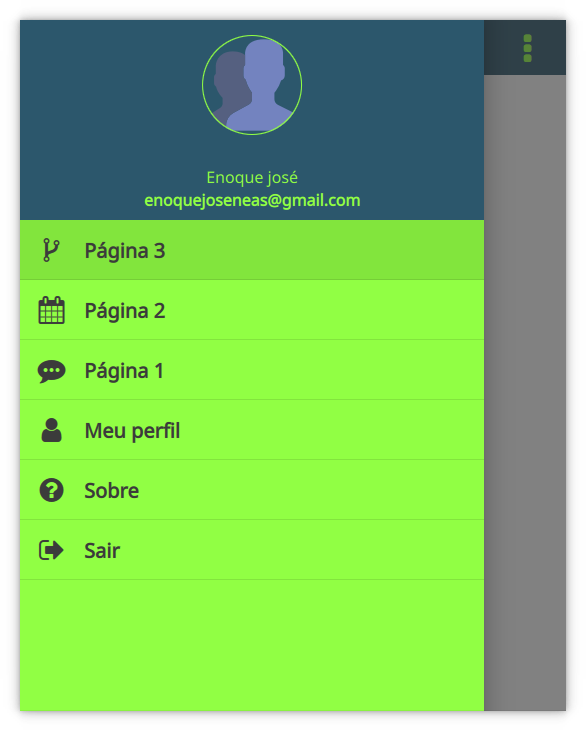
\includegraphics[width=8cm]{exemplo_menu_layout_em_pilha}
	\centering
	\caption{Lista de páginas exibidas no menu de layout em pilha}
\end{figure}

\begin{figure}[H]
	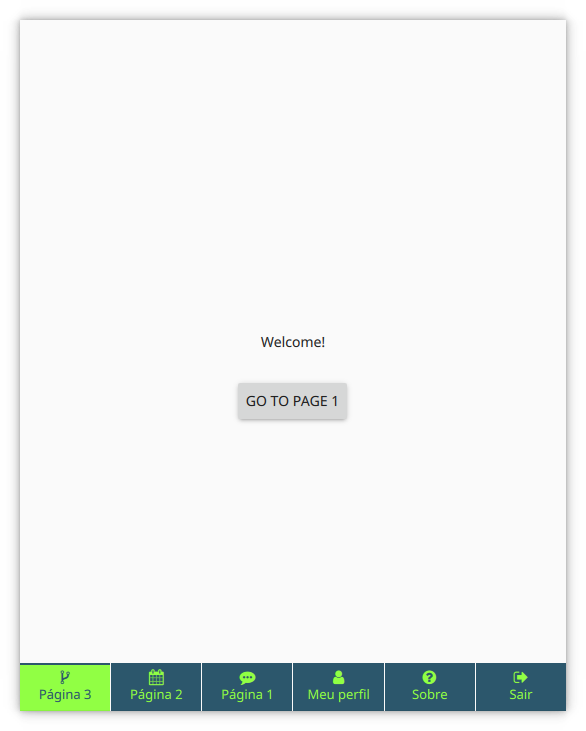
\includegraphics[width=8cm]{exemplo_menu_layout_em_linha}
	\centering
	\caption{Lista de páginas exibidas no menu de layout em linha}
\end{figure}


\subsection{Gerenciamento de plugins}\label{sec:solucao-desenvolvida}
A classe \textit{PluginManager} é responsável por carregar os plugins, basicamente, iterando os arquivos dentro do diretório \textit{plugins} e analisando as propriedades do arquivo de configuração de cada plugin. Em cada arquivo, o objeto verificará as definições de cada página (a partir do array \textit{pages}), transformando cada item em um objeto e adicionado em uma lista. Após ler todos os plugins, o array de objetos será persistido nas configurações da aplicação para que na próxima inicialização não precise iterar novamente o diretório, lendo as definições dos plugins das configurações. Os plugins serão recarregados após uma atualização do aplicativo ou quando a aplicação for executada em modo \textit{debug}.\par
A cada inicialização, será feito uma verificação da versão do aplicativo, que será persistida nas configurações na primeira execução do aplicativo e atualizada a cada \textit{release}. Se houver diferença entre versão em execução da versão salva na execução anterior, os plugins serão recarregados. Além disso, esta classe também é responsável por deletar todos os arquivos de cache contido no diretório de cache da aplicação a cada \textit{release}. Outra responsabilidade dessa classe, é a criação da tabela do plugin no banco de dados do aplicativo, se existir um arquivo \textit{plugin\_table.sql} no diretório do plugin. O banco de dados da aplicação será criado por outro objeto que controla as operações de persistência e será detalhado em outra seção. O diagrama a seguir, apresenta as operações e atributos da classe \textit{PluginManager}.

\begin{figure}[H]
	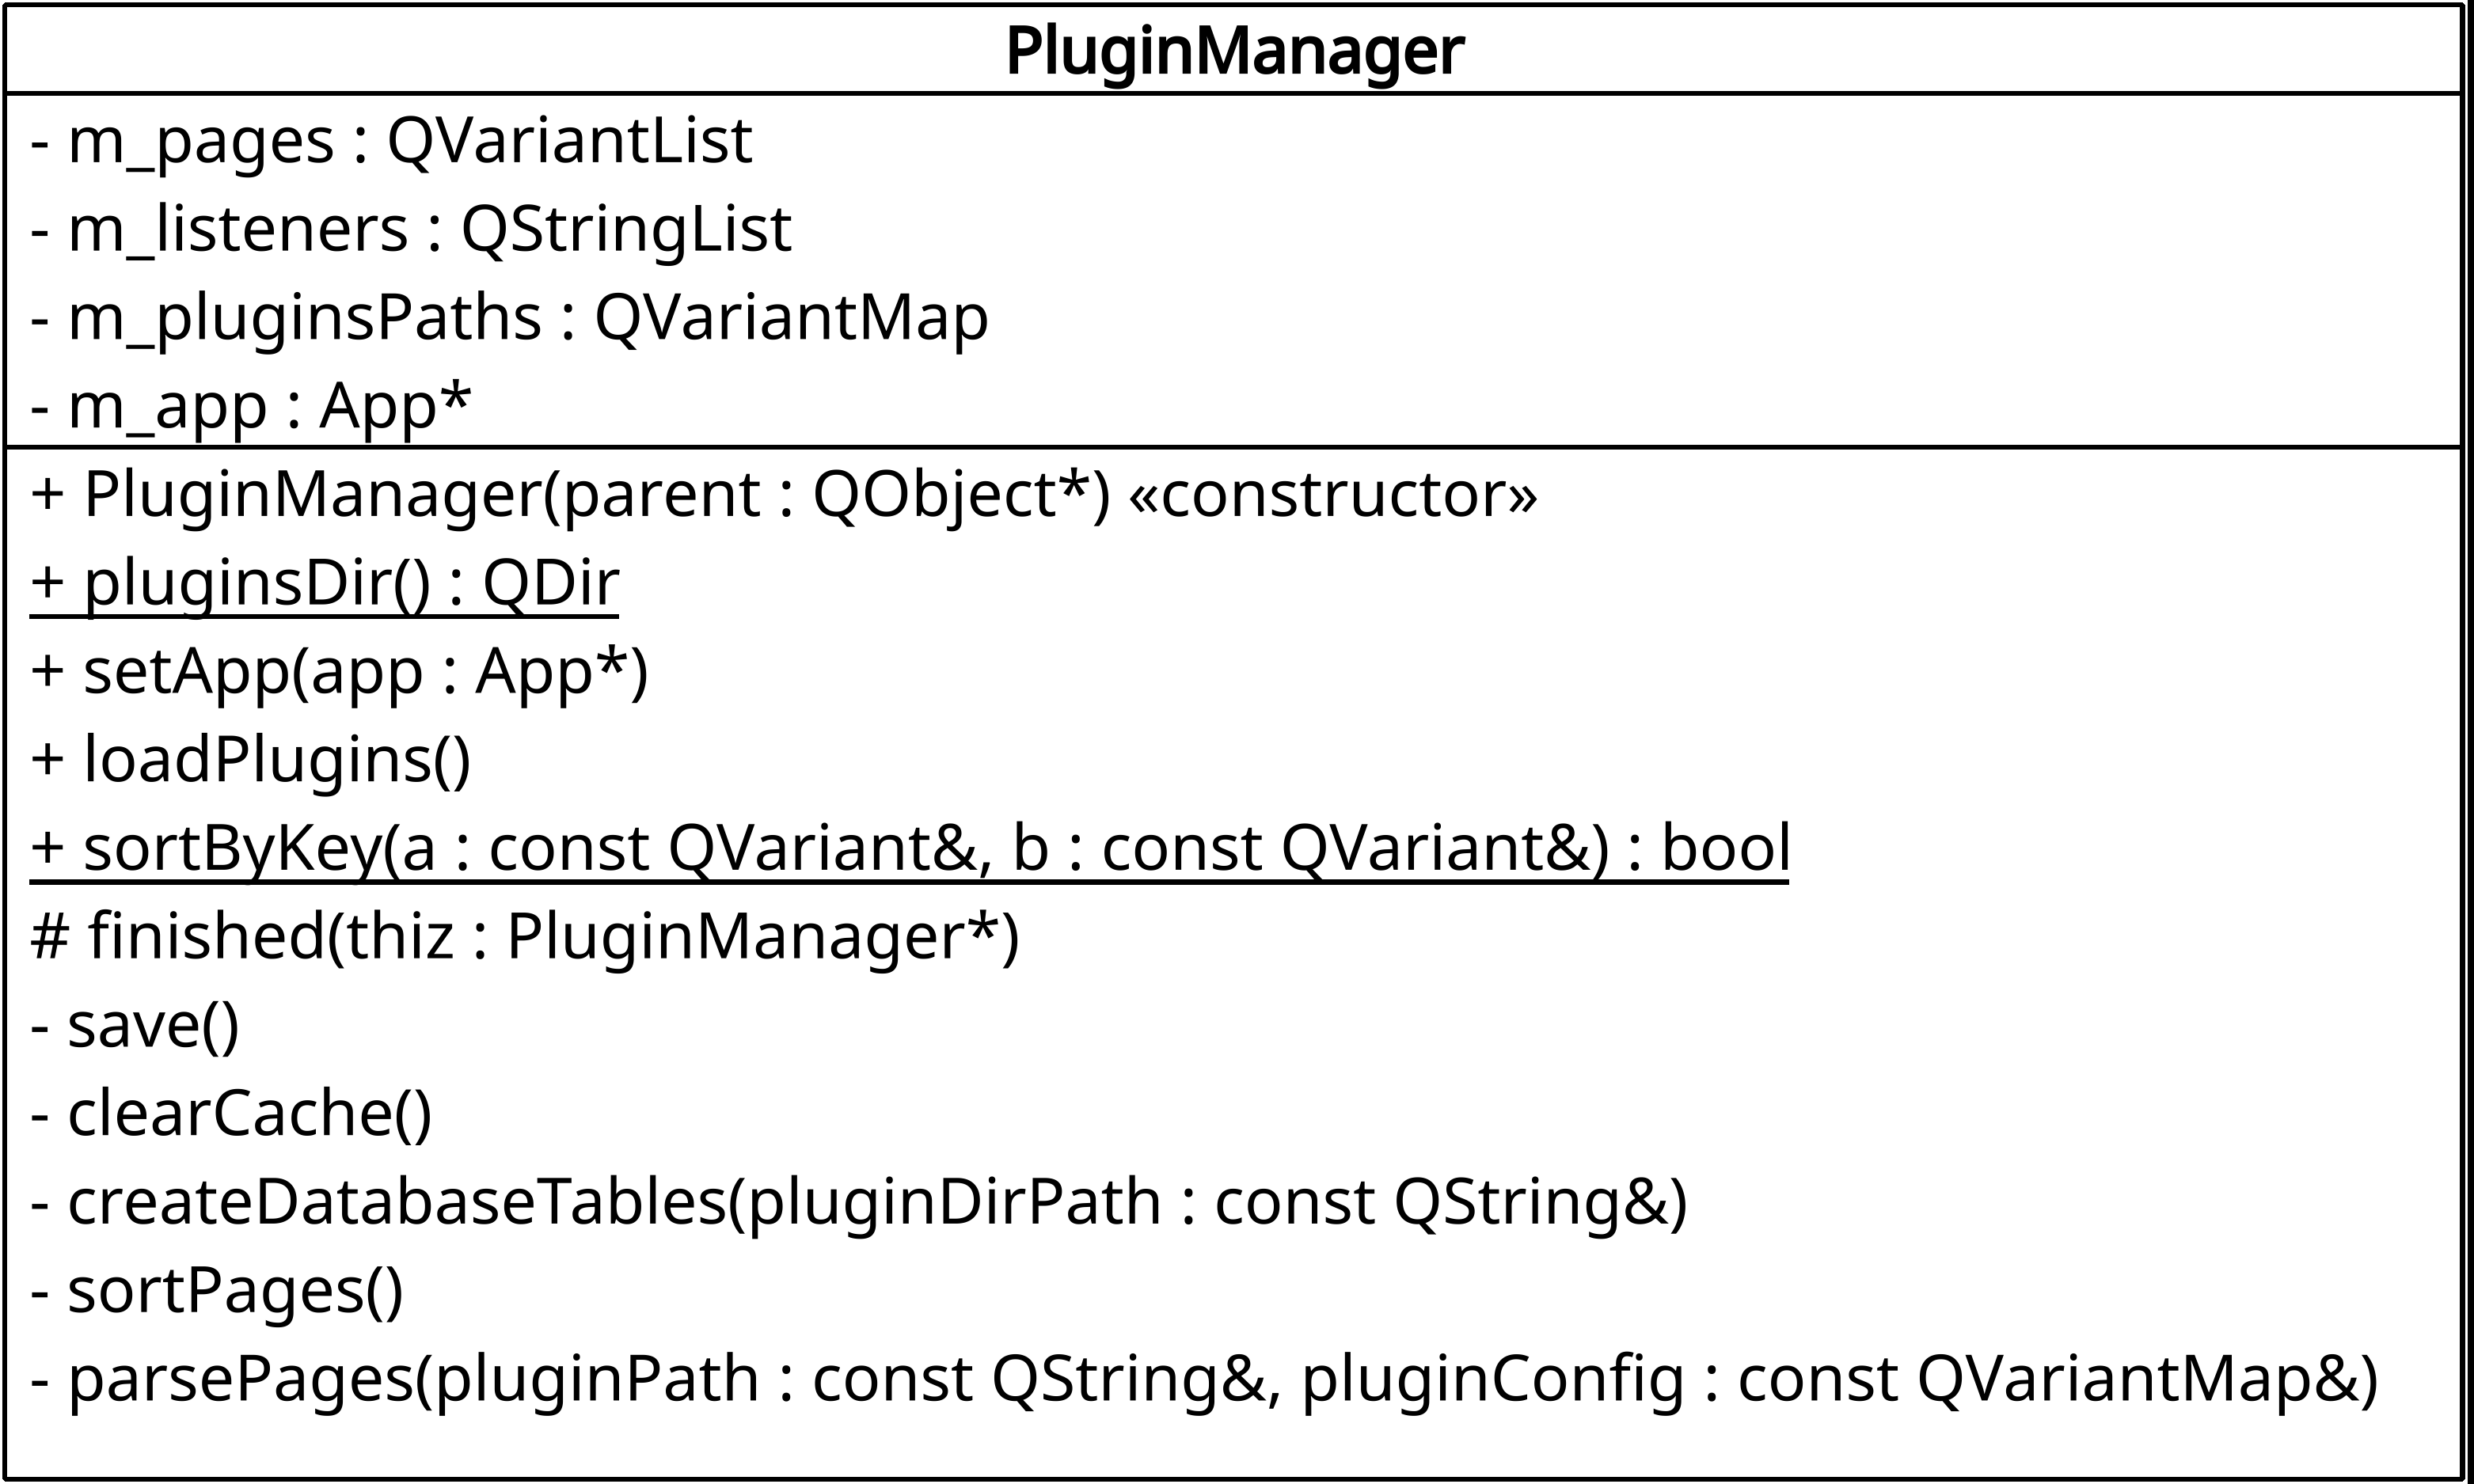
\includegraphics[width=8cm]{diagrama_de_classe_PluginManager}
	\centering
	\caption{Diagrama da classe PluginManager}
\end{figure}

O carregamento dos plugins será feito antes de instanciar qualquer componente visual, na invocação do método \textit{loadPlugins} feito pelo objeto \textit{App}. A instância de \textit{PluginManager} será destruída após o carregamento dos plugins para garantir baixo consumo de memória pelo aplicativo.


\subsection{A classe App}\label{sec:solucao-desenvolvida}
A classe \textit{App} é um componente importante nesta arquitetura, suas principais responsabilidades consiste de instanciar \textit{PluginManager}, carregar o arquivo \textit{config.json} que contém parâmetros da aplicação e gerenciar a persistência das configurações do aplicativo via \textit{QSettings}\footnote{https://doc.qt.io/qt-5/qsettings.html.}. \textit{App} será responsável por notificar os objetos da aplicação através do sinal \textit{eventNotify}, ela será instanciada na inicialização do aplicativo e registrada no contexto da aplicação identificada como \textit{App} para que os plugins possam invocar seus métodos públicos. Outra tarefa que corresponde a esta classe, é a criação de uma conexão com a atividade do aplicativo no android e no iOS para uso de notificações via push ou local. A aplicação poderá receber parâmetros de eventos como \textit{push notification} ou token de registro no \textit{Firebase}, quando o serviço de \textit{push} for utilizado. O registro do aplicativo no \textit{Firebase} e o recebimento de notificações via \textit{push} será realizado por objetos nativos de cada plataforma em um processo separado da aplicação. Em tempo de execução, as atividades (android \textit{Activity} e iOS \textit{AppDelegate}) passarão o token ou os argumentos recebidos do \textit{push} (título, mensagem, data de envio, etc.) para o aplicativo através de uma chamada ao método \textit{fireEventNotify} da classe \textit{App}. Quando isso ocorrer, \textit{App} notificará a aplicação através de dois eventos: \textit{newPushNotificationToken} e \textit{newPushNotification}. A figura abaixo apresenta o diagrama da classe \textit{App}.

\begin{figure}[H]
	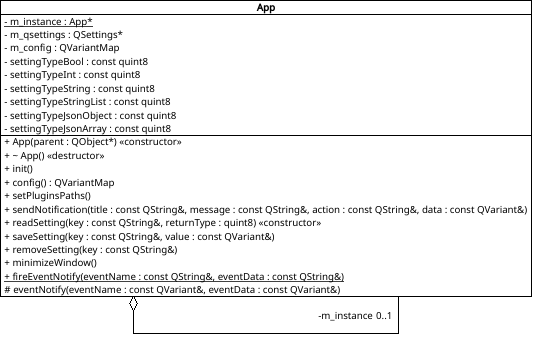
\includegraphics[width=8cm]{diagrama_de_classe_App}
	\centering
	\caption{Diagrama da classe App}
\end{figure}

\textit{App} é quem define o estilo de \textit{widgets} utilizado pelos componentes QML (Material, Universal, etc.). A definição do estilo deve ser feito pelo desenvolvedor no arquivo de configuração na propriedade \textit{applicationStyle} que será passado para um objeto \textit{QQuickStyle} do Qt na inicialização. Os possíveis valores para esta propriedade serão detalhados na seção que descreve o arquivo \textit{config.json}. O arquivo \textit{config.json} será registrado no contexto da aplicação como um objeto identificado como \textit{Config}. O objeto \textit{App} adicionará em \textit{Config} uma propriedade contendo o \textit{path} de cada plugin para facilitar o acesso aos arquivos no diretório de cada plugin. Por exemplo, considerando que \textit{Session} é um plugin, os arquivos em seu diretório poderão ser acessados da seguinte forma: \textit{Config.plugins.session + "File.qml"}. O objetivo dessa propriedade é fornecer aos plugins uma forma simplificada de acessar os arquivos em seu diretório, visto que os plugins serão colocados em diretórios virtuais nas plataformas \textit{mobile}: \textit{"assets://"} no android e "assets\_catalogs://" no ios. Quando executado em desktop, será utilizado o caminho absoluto de cada arquivo.


\subsection{Gerenciamento de configurações}
A arquitetura provê uma API simples e de alto nível para persistir dados utilizando o conceito \textit{chave-valor} através do objeto \textit{App}. Nesse modelo de persistência, a chave identifica o dado a ser armazenado e o valor é o dado propriamente dito. Os tipos de dados são: strings, números, objetos ou arrays e os métodos disponíveis podem ler, persistir ou deletar. As aplicações simples baseadas nesta arquitetura que não precisam de \textit{SQLITE}, poderão utilizar esse mecanismo para persistir dados no dispositivo. Os métodos disponíveis estão declarados na classe \textit{App} e poderão ser utilizados pelos plugins usando o objeto que será registrado no contexto da aplicação. Os métodos serão descritos a seguir e logo após, será apresentado um exemplo de como utilizá-los:
	\begin{itemize}
		\item \textit{readSetting}: Utilizado para ler um dado salvo utilizando uma string que identifique a informação a ser retornada. Por padrão, o tipo de retorno é string. Porém, se o dado não for string, o segundo parâmetro deve ser passado indicando o tipo específico a ser retornado. Os tipos podem ser especificados para evitar o uso de \textit{cast} no QML. Os tipos possíveis são:
		\begin{itemize}
			\item \textit{SettingTypeBool}: para retornar um valor booleano;

			\item \textit{SettingTypeInt}: para retornar um inteiro;

			\item \textit{SettingTypeStringList}: para retornar uma lista de strings;

			\textit{SettingTypeJsonObject}: para retornar um objeto;

			\item \textit{SettingTypeJsonArray}: para retornar um array de objetos.
		\end{itemize}

		\item \textit{saveSetting}: Utilizado para persistir alguma informação. Esse método é \textit{void} e possui dois parâmetros requeridos. O primeiro é uma string que identifica o dado a ser persistido, e o segundo, é o dado propriamente dito. O dado pode ser uma string, um valor numérico, um objeto ou array.

		\item \textit{removeSetting}: Utilizado para apagar alguma informação da configurações. Esse método requer apenas um parâmetro, uma string que identifica o dado a ser deletado.
	\end{itemize}

O código a seguir, apresenta um exemplo de persistência e leitura de dados usando o mecanismo \textit{chave-valor} a partir do objeto \textit{App}:

\begin{center}
\begin{lstlisting}[language=qml]
import QtQuick 2.8

Item {
    Component.onCompleted:{
		var foo = App.readSetting("foo")
		if (bar != foo)
		   App.saveSetting("foo",bar)
		App.removeSetting("bar")
    }
}
...
Item {
	...
	key:"bar"
	count:App.readSetting(key,App.SettingTypeInt)
	...
	Component.onCompleted:{ 
		App.saveSetting(key,++count)
	}
}
\end{lstlisting}
\captionof{lstlisting}{Exemplo de persistência através do objeto \textit{App}}
\end{center}


\subsection{Gerenciamento de eventos}
A classe \textit{App} dispõe o sinal \textit{eventNotify} que poderá ser utilizado pelos plugins como conector entre objetos. Este sinal possui dois parâmetros: o primeiro (\textit{eventName}) é uma string que identifica o evento e o segundo (\textit{eventData}), um objeto, string ou valor numérico contendo o dado ou argumento do evento a ser passado para os objetos ouvintes. Os objetos da aplicação podem disparar eventos da seguinte forma: \textit{App.eventNotify(nome-do-evento, argumento)}. Observadores devem criar uma conexão com este sinal utilizando o \textit{Connections} do \textit{Quick Controls}, especificando como \textit{target} o objeto \textit{App}. O código a seguir, apresenta um exemplo de uma conexão com este sinal:

\begin{center}
\begin{lstlisting}[language=qml]
import QtQuick 2.8
...
Connections {
    target:App
    onEventNotify:{
    	//eventData = o argumento do evento
        if (eventName == Config.events.foo)
            foo(eventData)
        //dispara outro evento, passando o valor
        //1000 como argumento do evento
        App.eventNotify(Config.events.bar,1000)
    }
}
\end{lstlisting}
\captionof{lstlisting}{Exemplo de conexão com o sinal \textit{eventNotify}}
\end{center}


\subsection{O Arquivo de Configuração}\label{sec:solucao-desenvolvida}
O arquivo \textit{config.json} presente na raiz do projeto é um componente importante desta arquitetura e contém as definições de configuração do aplicativo. No entanto, as informações desse componente não serão persistidas e o conteúdo (propriedades e valores) será passado para a aplicação como um objeto javascript global. As propriedades listadas a seguir, serão utilizadas por componentes internos e o desenvolvedor poderá adicionar outras propriedades quando for necessário compartilhar informações entre os plugins. Os plugins poderão ler as propriedades declaradas neste arquivo via \textit{Config.property\_name}. As propriedades difinidas inicialmente e utilizadas pela aplicação estão descritas a seguir:

\begin{itemize}
	\item \textit{applicationName} (string): O nome do aplicativo. Este valor será passado para o Qt na inicialização da aplicação. O valor dessa propriedade será utilizado para definir o nome dos arquivos de configuração (\textit{QSettings}) e do banco de dados SQLITE (quando houver);

	\item \textit{organizationName} (string): O nome da organização do aplicativo. Este valor também será passado para o Qt na inicialização do aplicativo e será utilizado para nomear e identificar o diretório de configurações e cache do aplicativo;

	\item \textit{organizationDomain} (string): O endereço de domínio da organização, por exemplo, \textit{qt.project.org}. O valor dessa propriedade será utilizado pelo Qt internamente;

	\item \textit{applicationStyle} (string): O nome do estilo a ser aplicado nos \textit{widgets} (\textit{Button}, \textit{TabBar}, \textit{ToolTip} etc.) do \textit{Quick Controls}. Os possíveis valores são: \textit{Material}, \textit{Universal} ou \textit{Default};

	\item \textit{forceEulaAgreement} (bool): Um valor booleano que indica se a aplicação deverá exigir do usuário confirmação de aceitação dos termos de uso para continuar usando o aplicativo. Esse valor só terá efeito se a propriedade \textit{showEula} for definida para \textit{true};

	\item \textit{hasLogin} (bool): Um valor booleano que indica se o aplicativo deverá carregar uma página de login na inicialização. Se for definido para \textit{true}, a aplicação irá utilizar a página que definiu (dentre os plugins) \textit{isLoginPage} para \textit{true};

	\item \textit{showEula} (bool): Um valor booleano que indica se a aplicação exibirá para o usuário uma página contendo os termos de uso do aplicativo. Caso seja setado para \textit{true}, o arquivo \textit{assets/eula.html} será carregado e exibido na primeira execução do aplicativo. Após o usuário ler e aceitar os termos de uso, o usuário irá para a página de login ou a \textit{home page}. No entanto, se essa propriedade for utilizada o desenvolvedor deverá escrever os termos de uso no arquivo \textit{assets/eula.html};

	\item \textit{showTabButtonText} (bool): Um valor booleano que indica se o título da página será exibida nos botões do menu em linha (\textit{TabButton} do \textit{Quick Controls}). Essa propriedade terá efeito somente quando a aplicação tiver usando o layout em linha;

	\item \textit{usesSwipeView} (bool): Um valor booleano que indica se o layout principal do aplicativo será em linha. Caso essa propriedade seja \textit{true}, o aplicativo utilizará o container \textit{SwipeView} do \textit{Quick Controls}. No entanto, o container responsável pelo layout em pilha (\textit{StackView}) ainda continuará disponível na aplicação, porém como container secundário. Um objeto fará o \textit{Binding} entre ambos, ocultando o \textit{SwipeView} quando alguma página for adicionada a pilha do \textit{StackView}. No \textit{SwipeView} o usuário poderá alternar entre as páginas deslizando horizontalmente;

	\item \textit{usesDrawer} (bool): Um valor booleano que indica se o menu lateral usado no layout em pilha, será instanciado. Essa propriedade terá efeito apenas no layout em linha, ou seja, se \textit{usesSwipeView} for \textit{true}, pois no layout em pilha ele será instanciado mesmo que o valor seja \textit{false}. O objetivo dessa propriedade é permitir que o desenvolvedor possa utilizar o menu lateral junto com o \textit{SwipeView}, intercalando as páginas que serão visíveis em cada um dos menus através das propriedades \textit{showInDrawer} e \textit{showInTabBar} na configuração das páginas de cada plugin;

	\item \textit{showDrawerImage} (bool): Um valor booleano que indica se a imagem do menu será carregada. Por padrão a imagem não será exibida. Se essa propriedade for definida para \textit{true}, a imagem definida em \textit{assets/drawer.jpg} será utilizada e o desenvolvedor poderá substituí-la por uma de sua preferência;

	\item \textit{restService} (object): Um objeto contendo as definições do serviço \textit{RESTful}, como url base e os parâmetros de autenticação básica (\textit{Basic Authentication}) usuário e senha. Os valores das propriedades \textit{userName} e \textit{userPass} serão convertidos em um \textit{hash} \textit{base64} e passado no cabeçalho de cada requisição HTTP. As seguintes propriedades são requeridas:

	\begin{itemize}
		\item \textit{userName} (string): O nome do usuário do serviço \textit{RESTful};

		\item \textit{userPass} (string): A senha de usuário do serviço \textit{RESTful};

		\item \textit{baseUrl} (string): A url base do serviço \textit{RESTful}. Essa propriedade será utilizada pelo objeto \textit{RequestHttp} nos métodos de requisições \textit{GET}, \textit{POST} etc. A sugestão é que o desenvolvedor adicione apenas o \textit{path} nos objetos que fazem requisições HTTP. Desta forma, se a url do \textit{web service} for modificada, basta alterar apenas no arquivo de configuração. Internamente, o objeto que realiza requisições concatenará o valor dessa propriedade com o \textit{path} passado no primeiro parâmetro dos métodos.
	\end{itemize}

	\item \textit{fontSize} (object): Um objeto com as definições de valores inteiros para os tamanhos de fonte a serem utilizadas em elementos textuais tais como o \textit{Label}. Essa propriedade possui quatro atributos: \textit{small}, \textit{normal}, \textit{large} e \textit{extraLarge};

	\item \textit{theme} (object): Um objeto com as definições de cores utilizada nos elementos visuais, tais como Botões, \textit{ToolBar}, \textit{TabBar}, cor de fundo das páginas e cor de fundo do \textit{drawer};

	\item \textit{events}: (array): Um array de strings com os eventos utilizados pelos plugins. Essa propriedade será utilizada por objetos e componentes internos para identificar de qual evento estão sendo notificados, a fim de padronizar os nomes dos eventos e reduzir a replicação de strings na aplicação. Essa propriedade poderá ser utilizado tanto em conexões com o sinal \textit{eventNotify} do objeto \textit{App} como pela API do \textit{Observer} disponibilizado pela arquitetura como alternativa para comunicação entre objetos através de eventos (será detalhado em um seção mais adiante). Componentes internos disparam eventos através do sinal \textit{eventNotify} usando a seguinte notação: \textit{App.eventNotify(Config.events.userProfileChanged, null)}. O objeto \textit{App} adicionará treze valores a essa propriedade que serão os identificadores de eventos internos. Porém, os valores podem ser utilizados pelos plugins para executarem ações específicas em dado momento. Os eventos adicionados pelo objeto \textit{App} serão descritos a seguir:

	\begin{itemize}
		\item \textit{cameraImageSaved} (string): Utilizado para notificar observadores de que uma imagem foi capturada pela câmera do dispositivo e salva localmente. A url da imagem salva será passado no argumento do evento;

		\item \textit{cancelSearch} (string): Utilizado pelo \textit{ToolBar} para indicar que o campo de busca não está ativo, para que a página corrente atualize o conteúdo para o usuário. O \textit{ToolBar} possui um campo texto para pesquisa e ficará visível quando a página alterar o valor da propriedade \textit{toolBarStatus} para \textit{"search"}. Essa funcionalidade permitirá que uma página filtre os resultados exibidos na sua \textit{view}, recebendo em um atributo string \textit{searchText} o valor digitado no campo. O usuário poderá cancelar a busca clicando em um botão voltar que ficará visível ao lado esquerdo do campo de busca e nesse momento, este evento será disparado;

		\item \textit{logoutApplication} (string): Utilizado pelo objeto \textit{UserProfile} para atualizar o status da propriedade \textit{isUserLoggedIn} para \textit{false} e em seguida carregar na página de login;

		\item \textit{newActionNotification} (string): Utilizado para notificar a aplicação quando o usuário clicar em uma notificação e o aplicativo ficar em \textit{foreground}, vale para notificações via \textit{push} e local. Esse evento será disparado pela atividade do Android (\textit{CustomActivity}) e pelo objeto \textit{QtAppDelegate} no iOS e repassado para a aplicação através do objeto \textit{App}. O argumento do evento (\textit{eventData}) conterá os dados da mensagem em uma string sendo necessário fazer o \textit{parsing} caso seja um objeto json;

		\item \textit{newPushNotification} (string): Utilizado sempre que uma notificação via \textit{push} chegar no dispositivo e o mesmo estiver em execução, em \textit{foreground} ou \textit{background}. Ele será disparado a partir dos serviços de notificação que executam em outro processo e serão repassados para a aplicação através de uma conexão entre o objeto java \textit{CustomAtivity} no android e o \textit{QtAppDelegate} no iOS. O argumento do evento (\textit{eventData}), conterá os dados da mensagem em uma string sendo necessário fazer o \textit{parsing} caso seja um objeto json;

		\item \textit{newPushNotificationToken} (string): Utilizado quando o registro no \textit{Firebase} for realizado com sucesso. Esse evento será disparado por objetos que executam em outro processo e serão passados para a aplicação através de uma conexão entre o objeto java \textit{CustomAtivity} no android e o \textit{QtAppDelegate} no iOS. O argumento do evento (\textit{eventData}) conterá o token em uma string;

		\item \textit{openDrawer} (string): Utilizado intermante para abrir o menu do layout em pilha quando o usuário clicar no botão de menu, posicionado no canto esquerdo do \textit{ToolBar}. O menu do layout em pilha fica oculto por padrão e o usuário poderá torná-lo visível arrastando da esquerda para a direita na janela do aplicativo;

		\item \textit{popCurrentPage} (string): Esse evento deverá ser disparado quando for necessário remover a página ativa da pilha do \textit{StackView}. Será disparado internamente pelo \textit{ToolBar} quando o usuário clicar no botão voltar (seta para a esquerda, exibido se a página definir a propriedade \textit{toolBarState} para \textit{"goBack"}) ou quando o botão \textit{back-button} do android for pressionado. O \textit{StackView} por exemplo, removerá a página da pilha quando este evento for emitido;

		\item \textit{appendOptionPage} (string): Esse evento pode ser utilizado para adicionar um novo item na lista de opções do menu. Esse evento poderá ser utilizado em ambos os layouts em pilha ou em linha e o argumento do evento deve ser um objeto contendo as propriedades de uma página utilizado no \textit{config.json} de um plugin;

		\item \textit{requestUpdateUserProfile} (string): Esse evento deve ser emitido para atualizar as informações ou dados do usuário no objeto \textit{UserProfile}. Por exemplo, uma página que permite editar os dados do usuário em um formulário, após o usuário atualizar alguma informação, a página poderá emitir esse evento passando como argumento um objeto contendo as informações do usuário no estilo \textit{chave-valor}. O objeto \textit{UserProfile} observará esse evento e salvará as informações localmente;

		\item \textit{initUserProfile} (string): Esse evento deve ser utilizado para inicializar o perfil do usuário após o login, recebendo um objeto json contendo as informações que serão persistidas localmente. O json deverá ser passado no argumento do evento, contendo no mínimo as propriedades \textit{id} e \textit{email}. Um exemplo de uso deste evento, pode ser feito pela página de login, após sucesso na autenticação. A página de login poderá emitir esse evento e passar como argumento o objeto retornado pelo serviço \textit{REST}. O objeto \textit{UserProfile} observará esse evento e quando o mesmo for emitido, salvará os dados do usuário na propriedade \textit{profile}. Em seguida, a propriedade \textit{isLoggedIn} será atualizada para \textit{true} e a \textit{home page} será carregada;

		\item \textit{setUserProfileData} (string): Esse evento também deve ser utilizado quando houver um perfil de usuário e permitirá adicionar ou atualizar uma informação no perfil do usuário. Logo, o argumento do evento deve conter a propriedade \textit{key} indicando o nome da propriedade a ser adicionada e \textit{value} contendo o respectivo valor. Por exemplo, o seguinte objeto pode ser utilizado como argumento deste evento: \textit{\{"key": "username", "value": "enoque"\}};

		\item \textit{userProfileChanged} (string): Esse evento será disparado pelo objeto \textit{UserProfile} sempre que ocorrer alguma atualização nos dados do usuário. No argumento do evento será passado uma referência para o objeto \textit{profile}.
	\end{itemize}
\end{itemize}


\subsection{Acesso a Rede (HTTP)}\label{sec:solucao-desenvolvida}
O primeiro requisito funcional provido nesta arquitetura é o acesso a rede para comunicação com serviços \textit{RESTful}. Para facilitar o uso de rede pelos plugins, foi criado uma classe C++ com suporte a autenticação básica, \textit{download} e \textit{upload} de arquivos, além de requisições via \textit{GET}, \textit{POST} e \textit{PUT}. O objetivo dessa classe é oferecer um componente rico em recursos, com bom desempenho e de alto nível para os plugins. Os plugins que utilizarem esse componente, receberão a resposta de cada requisição através de objetos json dispensando o uso de \textit{parsing}. Para simplificar o uso da API de rede, o desenvolvedor deverá adicionar na propriedade \textit{restService} no arquivo de configuração, a url do serviço \textit{RESTful} em \textit{baseUrl} e o nome e a senha do usuário em \textit{userName} e \textit{userPass} respectivamente. O objetivo é que o desenvolvedor utilize apenas o \textit{path} da url nos métodos de requisições. A subseção a seguir, descreve os detalhes da classe \textit{RequestHttp} seguido de exemplos de como instanciá-la e fazer requisições ao \textit{web service} do aplicativo.

\subsubsection{A classe RequestHttp}\label{sec:solucao-desenvolvida}
A classe \textit{RequestHttp} será registrada como um tipo QML no contexto da aplicação e para ser instanciada basta adicionar a diretiva \textit{import RequestHttp 1.0} e em seguida, declarar um objeto QML \textit{RequestHttp}. Internamente, os objetos inicializarão os atributos \textit{baseUrl} e nome de usuário e senha, porém, o desenvolvedor pode sobrescrevê-los quando for necessário. Essa classe utiliza \textit{QNetworkAccessManager} para gerenciar as operações de rede abstraindo para o aplicativo a interface de rede utilizada no dispositivo e \textit{QNetworkRequest} para encapsular os parâmetros da requisição. Os métodos e atributos disponíveis serão descritos a seguir, seguido de um exemplo de uso:

\begin{itemize}
	\item \textit{baseUrl} (string): atributo que define o endereço base do serviço \textit{REST}. Não precisa ser definido, pois será feito automaticamente no construtor do objeto. Porém, poderá ser utilizado pelo desenvolvedor quando a url definida no arquivo de configuração for diferente da url de destino de uma requisição específica. No entanto, é possível passar uma url absoluta nos métodos do objeto;

	\item \textit{authorizationUser} (string): atributo que define o nome do usuário do serviço \textit{REST}. Também não precisa ser definido, mas está disponível para que o desenvolvedor possa fazer requisições a uma url ou serviço com outro nome de usuário, além do que está definido no arquivo de configuração;

	\item \textit{authorizationPass} (string): atributo que define a senha do usuário do serviço \textit{REST}. Também não precisa ser definido, mas poderá ser modificado pelo desenvolvedor quando for preciso;

\begin{center}
\begin{lstlisting}[language=qml]
import QtQuick 2.8
import RequestHttp 1.0

RequestHttp {
	id:requestHttp
	baseUrl:"https://static.api.foo.com/"
	authorizationUser:"foo"
	authorizationPass:"bar.2018"
}
...
Item {
	Component.onCompleted:{
		var queryString = {
			arg1:"123",
			arg2:"321"
		}
		requestHttp.get("bar",queryString)
	}
}
\end{lstlisting}
% não está ficando centralizada
% \captionof{lstlisting} {Exemplo de uma requisição do tipo \textit{GET}}
\end{center}

	\item \textit{get}: método que realiza requisições do tipo \textit{GET} exigindo apenas a url de destino. Esse método possui dois parâmetros opcionais, o primeiro deles é um objeto do tipo \textit{chave-valor} e se for passado, adicionará a url uma \textit{query-string}. O segundo parâmetro opcional é também um objeto e pode ser passado quando for necessário adicionar dados no cabeçalho da requisição. O código a seguir, apresenta um exemplo de uso desse método:
\begin{center}
\begin{lstlisting}[language=qml]
import QtQuick 2.8
import RequestHttp 1.0

RequestHttp {
	id:requestHttp
}
...
Item {
	Component.onCompleted:{
		var queryString = {
			someKey:"foo",
			paginate:listView.count
		}
		//...foo?someKey=foo&paginate=16
		requestHttp.get("foo",queryString)
	}
}
\end{lstlisting}
% não está ficando centralizada
% \captionof{lstlisting} {Exemplo de uma requisição do tipo \textit{GET}}
\end{center}

	\item \textit{post}: método que realiza requisições do tipo \textit{POST} exigindo a url de destino e o dado a ser postado em formato string. O terceiro parâmetro desse método é opcional e pode ser passando quando for necessário adicionar dados no cabeçalho da requisição. O código a seguir, apresenta um exemplo de uso desse método:
\begin{center}
\begin{lstlisting}[language=qml]
import QtQuick 2.8
import RequestHttp 1.0
	
RequestHttp {
	id:requestHttp
}
...
Item {
	Component.onCompleted:{
		var postData = JSON.stringfy({
			someKey:"bar",
			email:textField.text
		})
		requestHttp.post("bar",postData)
	}
}
\end{lstlisting}
% não está ficando centralizada
% \captionof{lstlisting}{Exemplo de uma requisição do tipo \textit{POST}}
\end{center}

	\item \textit{uploadFile}: realiza uma requisição do tipo \textit{POST} ou \textit{PUT} exigindo a url de destino e um array de strings contendo os endereços dos arquivos locais a serem enviados para o servidor. A requisição será do tipo \textit{multipart-formdata} e do tipo \textit{POST} (por default). O terceiro parâmetro (booleano, default \textit{false}) pode ser passado quando for necessário utilizar o método \textit{PUT}. Já o último parâmetro, poderá ser passado quando for necessário adicionar dados no cabeçalho da requisição. Após invocar esse método, o sinal \textit{uploadFinished} será emitido para cada arquivo enviado. Durante o envio de cada arquivo, será emitido o sinal \textit{uploadProgressChanged} contendo os bytes do arquivo (local) e o total de bytes já enviados para o servidor. O código a seguir, apresenta um exemplo de uso desse método:
\begin{center}
\begin{lstlisting}[language=qml]
import QtQuick 2.8
import RequestHttp 1.0
	
RequestHttp {
	id:requestHttp
}
...
Item {
	Component.onCompleted:{
		var files = [
			"/data/app/myapp/files/img1.png",
			"/data/app/myapp/files/img2.png"
		]
		requestHttp.upload("bar",files)
	}
}
\end{lstlisting}
% não está ficando centralizada
% \captionof{lstlisting}{Exemplo de uma requisição de \textit{upload} de arquivos}
\end{center}

	\item \textit{downloadFile}: realiza uma requisição do tipo \textit{GET} exigindo apenas uma lista de urls de arquivos a serem baixados para o dispositivo. Por padrão, os arquivos serão salvos no diretório público de \textit{downloads} no dispositivo. No entanto, o segundo parâmetro \textit{saveInAppDirectory} (booleano, default \textit{false}) pode ser utilizado para alterar o diretório de destino dos arquivos para uma pasta interna do aplicativo. Após invocar esse método, para cada arquivo salvo, o sinal \textit{downloadFileSaved} será emitido passando o \textit{path} do arquivo salvo localmente. Durante o download de cada arquivo, o sinal \textit{downloadProgressChanged} será emitido passando dois argumentos, o primeiro indica o total de bytes do arquivo que está sendo baixado e o segundo, um valor inteiro indicando os bytes que já foram baixados. O código a seguir, demonstra um exemplo de requisição para download de arquivos:
\begin{center}
\begin{lstlisting}[language=qml]
import QtQuick 2.8
import RequestHttp 1.0
	
RequestHttp {
	id:requestHttp
}
...
Item {
	Component.onCompleted:{
		var urls = [
			"https://.../files/f1.png",
			"https://.../files/f2.png"
		]
		requestHttp.downloadFile(urls)
	}
}
\end{lstlisting}
% não está ficando centralizada
% \captionof{lstlisting}{Exemplo de uma requisição de \textit{upload} de arquivos}
\end{center}

\end{itemize}

Os métodos descritos anteriormente são todos \textit{void}, assíncronos e declarados como \textit{Q\_INVOKABLE} \footnote{htps://doc.qt.io/qt-5/qtqml-cppintegration-exposecppattributes.html} para permitir o uso dos métodos em componentes QML, como é o caso do componente \textit{RequestHttp}. Para obter a resposta de uma requisição, é preciso criar uma conexão com o sinal \textit{finished}. Esse sinal será emitido por todos os métodos descritos anteriormente se não houver erros no pedido e logo após o envio da resposta pelo servidor. O sinal \textit{finished} passará dois argumentos, \textit{statusCode}, um valor inteiro indicando o status da resposta (200, 400, 500, etc.) e \textit{response} contendo o dado enviado pelo servidor. Se a resposta enviada pelo servidor for um json válido (objeto ou array), \textit{response} conterá um objeto ou array, caso contrário, uma string contendo o dado bruto.\par

O sinal \textit{error} será emitido quando houver erros em um pedido e passará dois argumentos, \textit{statusCode} (integer) indicando o código HTTP correspondente ao erro, e \textit{message} (string) contendo a mensagem do erro.\par

A propriedade \textit{status} (integer) declarada como \textit{Q\_PROPERTY} indicará o \textit{status} atual de uma requisição. Essa propriedade pode ser comparada com qualquer uma das seguintes meta-propriedades (útil para fazer \textit{bindings} com outros objetos):

\begin{itemize}
	\item \textit{Error}: indica um erro no pedido, quando o servidor não responder ou o status da requisição for zero;

	\item \textit{Finished}: indica que a requisição terminou e será setada em \textit{status} antes da emissão do sinal \textit{finished};

	\item \textit{Loading}: indica que a requisição está em andamento ou carregando;

	\item \textit{Ready}: indica que a requisição está pronta, será setada em \textit{status} no construtor do objeto \textit{RequestHttp} e logo após a emissão do sinal \textit{finished}.
\end{itemize}

\begin{center}
\begin{lstlisting}[language=qml]
import RequestHttp 1.0 
	
RequestHttp {
	id:request
}
...

Button {
	text:"Submit"
	enabled:request.status == request.Ready
	onClicked:request.get("foo",{"bar":1})
}
...
\end{lstlisting}
\captionof{lstlisting}{Exemplo de \textit{Bind} com o status de uma requisição}
\end{center}


O diagrama a seguir, apresenta os atributos e métodos da classe \textit{RequestHttp}:

\begin{figure}[h]
	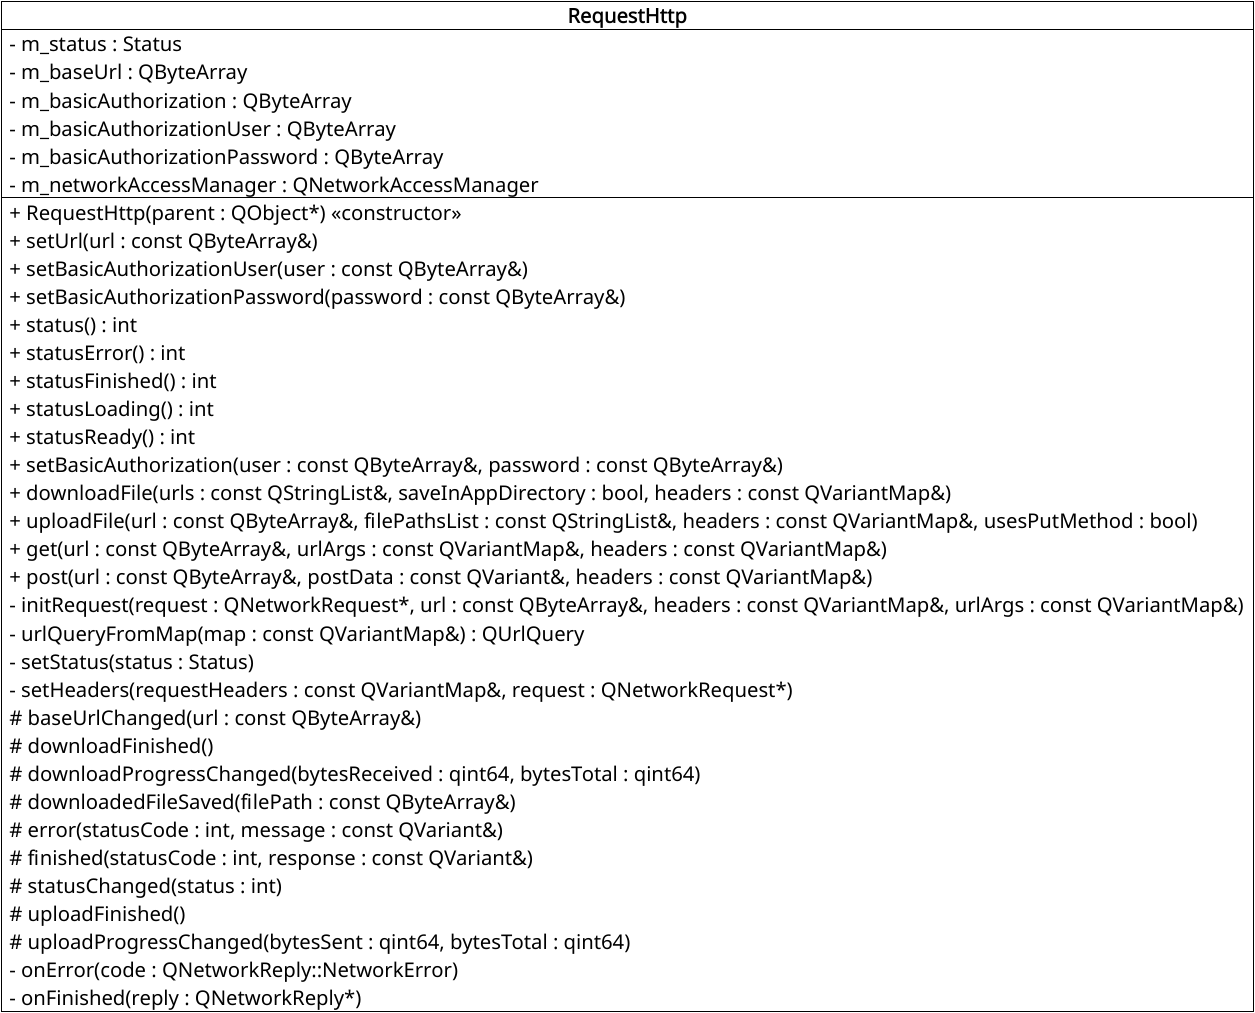
\includegraphics[width=8cm]{diagrama_de_classe_RequestHttp}
	\centering
	\caption{Diagrama da classe \textit{RequestHttp}}
\end{figure}


\subsection{Persistência de Dados}\label{sec:solucao-desenvolvida}
Persistência de dados é o segundo requisito funcional disponibilizado nesta arquitetura e visa fornecer aos plugins a possibilidade de persistir dados em um banco \textit{SQLITE} e o funcionamento \textit{offline} do aplicativo. Cada plugin pode criar uma ou mais tabelas no banco de dados e realizar as operações de inserção, atualização e busca de dados em suas tabelas, basta importar o componente \textit{Database} com a diretiva \textit{import Database 1.0} e utilizá-lo em um componente QML. Para criar as tabelas no banco de dados do aplicativo, o plugin deve fornecer um arquivo \textit{plugin\_table.sql} contendo os comandos de criação, alteração ou remoção das tabelas. A cada \textit{release}, esse arquivo será carregado e executado como uma \textit{query} sql permitindo aos plugins atualizar as tabelas (adicionar, remover ou modificar as colunas) quando for necessário.\par

Para gerenciar as operações de banco de dados, foi criado uma classe C++ chamada \textit{Database} que encapsula em métodos de alto nível as operações necessárias para criar o banco de dados, conectar e executar as operações sql. No entanto, essa classe não será utilizada pelos plugins diretamente, foi criado outra classe chamada \textit{DatabaseComponent} que agrega uma instância de \textit{Database} e delega as operações para esse objeto e fornece alguns recursos para simplificar ainda mais a persistência de dados. As subseções a seguir apresentam detalhes de ambas as classes \textit{Database} e \textit{DatabaseComponent}.

\subsubsection{A classe Database}\label{sec:solucao-desenvolvida}
A classe \textit{Database} é responsável por criar o banco de dados \textit{SQLITE} na primeira execução do aplicativo se houver necessidade, ou seja, se algum plugin dispor de um arquivo \textit{plugin\_table.sql} em seu diretório. Se nenhum plugin fornecer esse arquivo, o banco de dados \textit{SQLITE} não será criado. A classe \textit{Database} utiliza as classes \textit{QSqlDatabase} para criação e conexão com o banco de dados e as classes \textit{QSqlQuery} e \textit{QSqlRecord} para as realizar \textit{querys} e retornar os resultados das cosultas. Os métodos principais desta classe serão descritos a seguir:

\begin{itemize}
	\item \textit{select}: esse método pode ser utilizado para recuperar dados de uma tabela através de uma consulta \textit{sql} e possui três parâmetros, o primeiro é nome da tabela onde será feito a consulta, o segundo é um objeto contendo os parâmetros da consulta (condição \textit{where}) no estilo \textit{nome-da-coluna.valor}, e o último parâmetro, um outro objeto contendo argumentos adicionais, tais como \textit{limit}, \textit{offset} e \textit{order by}. Esse método retornará uma lista de objetos resultante da consulta, e cada objeto contido na lista é composto de \textit{nome-da-coluna.valor}. Se a consulta não for efetuada com sucesso, será retornado uma lista vazia;

	\item \textit{insert}: esse método pode ser utilizado para inserir dados em uma tabela e os parâmetros requeridos são: o nome da tabela onde será feito a inserção e um objeto no estilo \textit{nome-da-coluna.valor} contendo os dados a serem persistidos. Se a inserção for efetuada com sucesso e a tabela possuir uma coluna auto-incrementada como chave-primária o valor incrementado será retornado. Caso contrário, não possuir a coluna auto-incrementada, retornará o valor inteiro 1 (um) ou, retornará zero se houver erros na inserção;

	\item \textit{remove}: esse método pode ser utilizado para deletar um ou mais registros em uma tabela e três parâmetros são requeridos: o primeiro é o nome da tabela onde será feito a remoção, o segundo é um objeto contendo os argumentos ou filtros da \textit{query} no estilo \textit{nome-da-coluna.valor}. O terceito parâmetro é opcional e pode ser passado para customizar o operador de comparação para cada par \textit{nome-da-coluna.valor} no segundo parâmetro. Por default, será utilizado o operador de igualdade ("=");

	\item \textit{update}: esse método pode ser utilizado para atualizar um ou mais registros em uma tabela específica. Os parâmetros desse método são basicamente os mesmos do método \textit{remove} descrito no item anterior, com uma adição, o parâmetro \textit{updateData}, um objeto contendo os dados a serem atualizados também no estilo \textit{nome-da-coluna.valor};

	\item \textit{queryExec}: esse método pode ser utilizado para realizar uma consulta sql a partir de uma string passada como parâmetro. O valor booleano \textit{true} será retornado se a \textit{query} for efetuada com sucesso, caso contrário \textit{false}. O resultado da consulta se houver, deverá ser obtido através do método \textit{resultSet} descrito a seguir;

	\item \textit{resultSet}: esse método pode ser utilizado para recuperar um conjunto de dados resultante da última consulta sql efetuada, por exemplo, após a chamada ao método \textit{queryExec}. O tipo de retorno é uma lista de objetos no estilo \textit{nome-da-coluna.valor}. O método \textit{select} por exemplo, utiliza esse método como retorno da consulta efetuada internamente. Esse método possui um parâmetro opcional que deve ser utilizado quando a tabela a qual a última consulta efetuada for do tipo \textit{meta\_key.meta\_value} para que a chave do objeto seja a chave na tabela e o valor, o dado contido em meta\_value;
\end{itemize}

É importante destacar, que essa classe implementa o \textit{singleton}, e será instanciada na inicialização da aplicação pelo objeto \textit{pluginManager}. Se múltiplos plugins realizarem operações sql, eles utilizarão a mesma instância dessa classe. O diagrama a seguir apresenta os atributos e métodos da classe \textit{Database}.

\begin{figure}[h]
	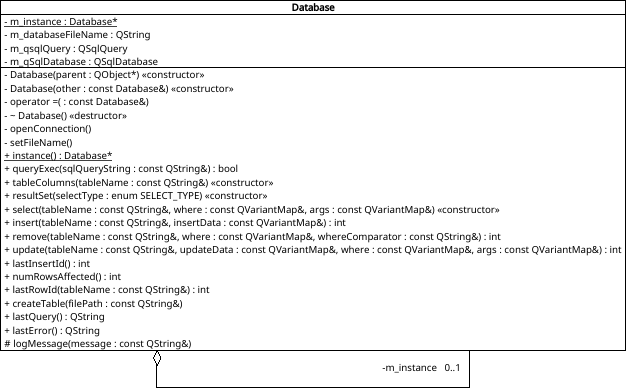
\includegraphics[width=8cm]{diagrama_de_classe_Database}
	\centering
	\caption{Diagrama da classe Database}
\end{figure}

\subsubsection{A classe DatabaseComponent}\label{sec:solucao-desenvolvida}
A classe \textit{DatabaseComponent} foi criada com o objetivo de fornecer um componente de alto nível que simplificasse para os plugins as operações em uma tabela específica. Essa classe será registrada no contexto da aplicação como um tipo QML com o nome de "\textit{Database}" e permitirá aos plugins utilizarem como componentes QML. \textit{DatabaseComponent} agrega uma instância da classe \textit{Database} e delega as operações para esse objeto. No entanto, ela possui alguns atributos declarados como \textit{Q\_PROPERTY} que permitem aos plugins informar o nome da tabela no banco de dados, uma coluna chave-primária do tipo string (quando a chave-primária não for numérica auto-incrementada), além de colunas que guardam objetos json. As colunas json evitam a realização de \textit{parsing} nas views ou \textit{delegates} para objetos agregados, sendo retornados já convertidos em objetos ou arrays.\par

Outro atributo \textit{totalItens} manterá atualizado o número de registros na tabela para fins de comparação com o número de itens disponível no serviço \textit{REST}, útil para paginação de dados na \textit{view}. O diagrama a seguir, apresenta os atributos e métodos dessa classe:

\begin{figure}[H]
	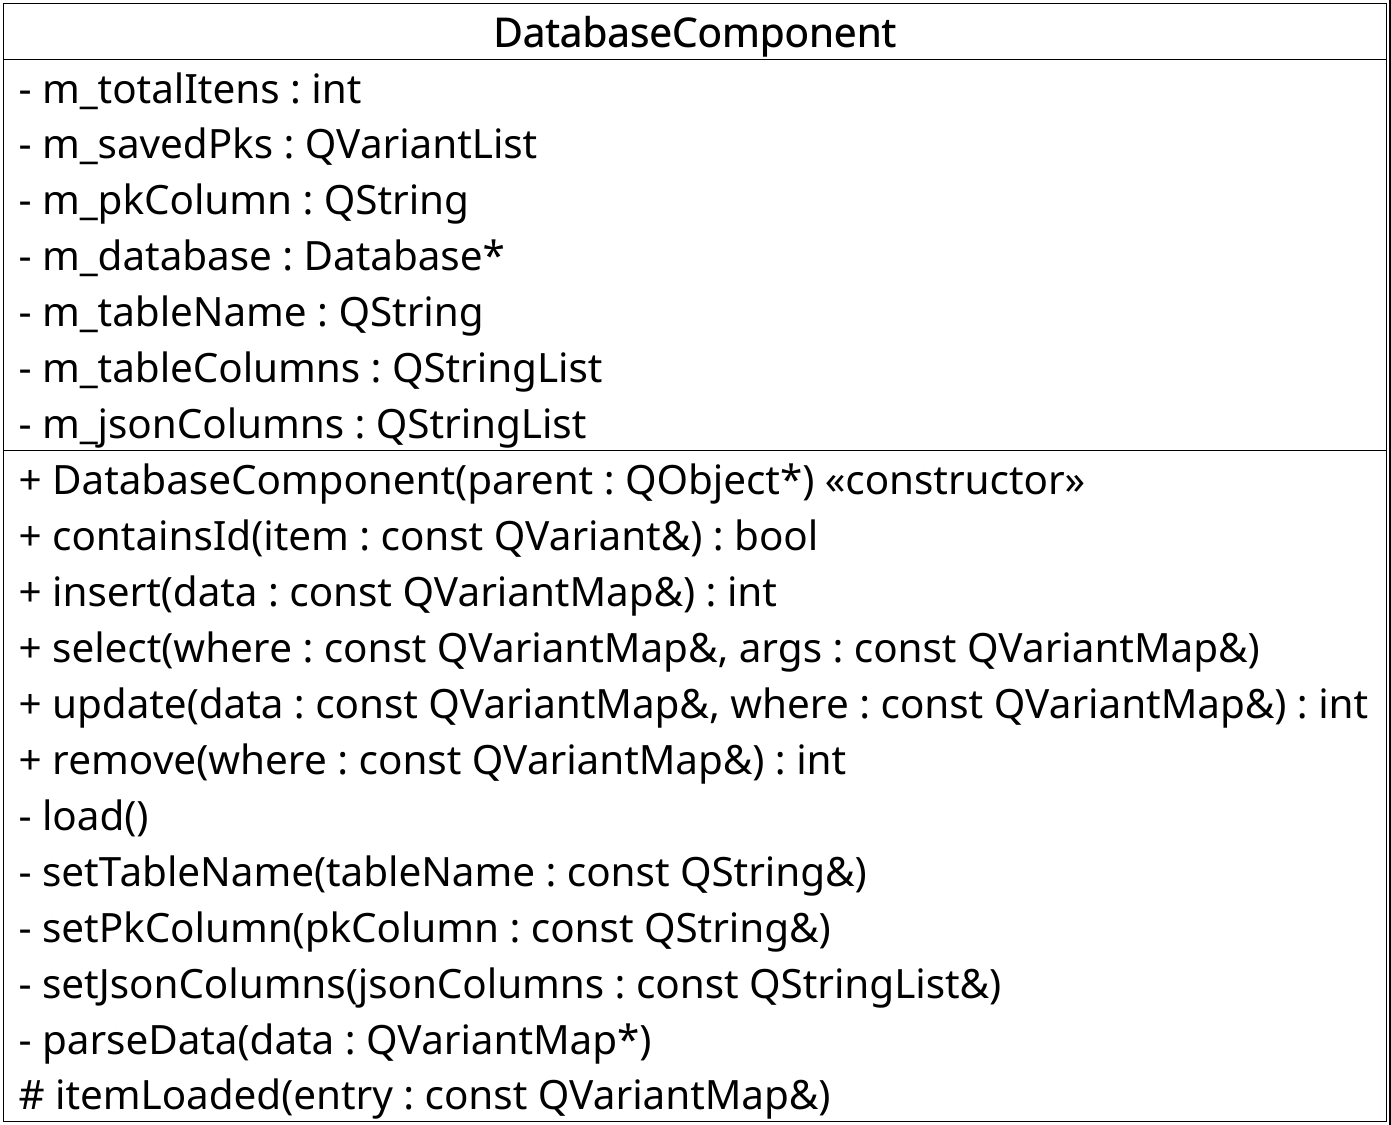
\includegraphics[width=8cm]{diagrama_de_classe_DatabaseComponent}
	\centering
	\caption{Diagrama da classe DatabaseComponent}
\end{figure}

É importante destacar que os métodos de busca, inserção, remoção e atualização foram simplificados para que os objetos informem apenas os parâmetros do método sem o nome da tabela. Outro recurso importante desse componente é que o método de busca é assíncrono e os resultados de uma busca, quando houver, serão retornados através do sinal \textit{itemLoaded} que passará como argumento um objeto no estilo \textit{nome-da-coluna.valor}. \textit{DatabaseComponent} possui ainda o método \textit{containsId} que verifica se um item (pela chave primária) já está salvo localmente e pode ser útil para sincronizar com a \textit{view} os itens já baixados do serviço \textit{REST}. O código a seguir, apresenta um exemplo de como um plugin poderá utilizar \textit{DatabaseComponent} para persistir dados em uma tabela:

\begin{center}
\begin{lstlisting}[language=qml]

import Database 1.0
...
Database {
	id:database
	jsonColumns:["source"]
	tableName:"news"
	pkColumn:"title"
	onItemLoaded:listViewModel.append(entry)
}
...
Item {
	Component.onCompleted:{
		var args = {
			title:"GNU is not Unix!",
			message:"GNU is an operating...",
			datetime:"2017-12-30T14:29:33"
			source:{
				url:"https://foo.com/api",
				code:"foo",
				value:"bar"
			}
		}
		database.insert(args)
	}
}
...
\end{lstlisting}
\captionof{lstlisting}{Exemplo de como utilizar \textit{DatabaseComponent}}
\end{center}


\subsection{Notificações do Aplicativo}
O terceiro requisito funcional disponibilizado nesta arquitetura é o envio de notificação ao usuário do aplicativo e consiste de notificações via \textit{push} e local. As notificações via \textit{push} é suportado apenas no Android e iOS e as notificações locais é suportado nos dispositivos móveis além de linux desktop e MacOS. As notificações podem ser utilizadas para alertar o usuário de algum evento na aplicação e pode conter um título, uma descrição e nas plataformas mobile, pode vibrar o dispositivo e emitir um som. Outro recurso disponibilizado nas notificações é a possibilidade de adicionar algum dado extra em cada notificação. Esse dado deve ser um objeto \textit{chave.valor} e o valor pode ser tanto uma string como um valor numérico ou, outro objeto ou array. As notificações locais serão enviadas pela própria aplicação via chamada de método e as notificações via \textit{push} através do \textit{Firebase}. As subseções a seguir, descrevem detalhes de cada tipo de notificação.

\subsubsection{Notificações via push}
O suporte a notificações via \textit{push} já está configurado na arquitetura e o que o desenvolvedor deve fazer para enviar mensagens via \textit{push} é criar um projeto no \textit{Firebase}, exportar o arquivo \textit{google-services.json} e adicioná-lo no diretório \textit{android} e o arquivo \textit{google-services.xml} correspondente ao iOS no diretório \textit{ios}, substituindo os arquivos existentes, ambos criados como exemplo. É importante destacar que o \textit{package name} do aplicativo adicionado no \textit{AndroidManifest.xml} e o \textit{CFBundleIdentifier} no \textit{Info.plist} do iOS, devem ser o mesmo utilizado ao criar o projeto no \textit{Firebase}. Caso contrário, ocorrerá um erro ao construir o APK ou IPA, pois as bibliotecas correspondentes ao serviço de \textit{push} (adicionadas ao projeto durante o \textit{build}) farão um \textit{parsing} dos arquivos e abortará a compilação caso ocorra algum erro. No android, o \textit{package name} deve ser adicionado manualmente no arquivo \textit{build.gradle} presente no diretório \textit{android} na propriedade \textit{defaultConfig.applicationId}.\par

No android, o funcionamento de \textit{push notification} requer duas classes java que serão instanciadas na inicialização do aplicativo e funcionarão como dois serviços. Essas classes já estão na arquitetura e o desenvolvedor não precisa modificá-las. O primeiro serviço registra o dispositivo no \textit{Firebase} e retorna um token. Quando isso ocorrer, o token será passado para a aplicação através do sinal \textit{eventNotify} do objeto \textit{App}. O segundo serviço é um \textit{listener} de notificações via \textit{push} e ficará em execução mesmo que a aplicação seja fechada. Ao enviar uma notificação utilizando o console do \textit{Firebase} ou através de algum \textit{web service}, as notificações serão recebidas nesse serviço e enviadas para o \textit{system tray} automaticamente. Se o aplicativo estiver em execução, a notificação será encaminhada para o aplicativo em um objeto json contendo todos os dados da mensagem: o título, a data e a hora de envio e o dado de \textit{payload} (um dado adicional não visível enviado na mensagem).\par

No iOS, o arquivo \textit{QtAppDelegate.mm} presente no diretório \textit{ios} realizará o registro do dispositivo no \textit{Firebase} e contém um método que receberá as notificações via \textit{push} e re-encaminhará para a aplicação usando o mesmo sinal utilizado no android. Em ambas as plataformas, o token será passado para a aplicação através do evento \textit{newPushNotificationToken} e as mensagens de push, no evento \textit{newPushNotification}. Se a aplicação estiver em execução e o usuário clicar em uma notificação colocando o aplicativo em foreground, o evento \textit{newActionNotification} será disparado passando como argumento do evento os dados de \textit{payload} da mensagem.\par

A arquitetura dispõe do plugin de exemplo \textit{Listeners} que contém o componente \textit{PushNotificationRegister.qml}. Esse componente demostra um exemplo de como obter o token de registro no \textit{Firebase} e enviar para o serviço \textit{REST}, destruindo o componente (para otimizar consumo de memória) quando o token for recebido com sucesso pelo servidor.

\begin{center}
\begin{lstlisting}[language=qml]
import QtQuick 2.8

Connections {
    target: App
    onEventNotify:{
		var e
		e = Config.events.newPushNotificationToken
		if (e == eventName) {
			//enviando o token para o web service
			//eventData eh o argumento do evento
			//contendo uma string com o token
			sendTokenToServer(eventData)
		}
	}
}
\end{lstlisting}
\captionof{lstlisting}{Exemplo de como acessar o token do \textit{Firebase}}
\end{center}

\subsubsection{Notificações local}
Para gerenciar as notificações locais, foi criado a classe \textit{Notification} que abstrai a plataforma e dispõe de um método para enviar uma notificação para a área de notificações do sistema em execução. Essa classe será instanciada na inicialização do aplicativo e registrada no contexto da aplicação para que os plugins possam invocar o método \textit{Notification.show}, passando o título e a mensagem da notificação e opcionalmente um objeto contendo o argumento a ser passado para a aplicação quando o usuário clicar na notificação. Quando o usuário clicar na notificação, o aplicativo ficará em \textit{foreground} (caso não esteja) e o argumento da notificação será passado para o objeto \textit{App} que notificará a aplicação via \textit{eventNotify} contendo em \textit{eventName} a string \textit{newActionNotification} e em \textit{eventData}, o argumento passado no método \textit{show}. O código a seguir, apresenta um exemplo de como exibir uma notificação local por algum objeto de um plugin, passando um título, uma mensagem e um objeto como argumento.

\begin{center}
\begin{lstlisting}[language=qml]
import QtQuick 2.8

Item {
    Component.onCompleted:{
		var title = "Novo item carregado!"
		var message = "Clique para visualizar!"
		var argument = {
			key:"foo",
			value:"bar"
		}
		Notification.show(title,message,argument)
	}
}
\end{lstlisting}
\captionof{lstlisting}{Exemplo de como exibir uma notificação local}
\end{center}


\subsection{Comunicação entre os objetos e plugins}
% Esta seção descreverá o processo de comunicação entre objetos no aplicativo e o uso correto dos eventos...
O quarto requisito funcional desta arquitetura é a disponibilização de um mecanismo de comunicação entre objetos e plugins facilitado. A seção 4.9 descreveu o uso do sinal \textit{eventNotify} do objeto \textit{App}, utilizado por componentes internos e pelos plugins disponibilizados como exemplo na arquitetura. Porém, esse não é o único mecanismo de comunicação disponibilizado, a arquitetura dispõe de uma implementação em C++ do padrão de projeto \textit{Observer} baseado em categorias de eventos. A categoria, neste caso, é uma string que identifica um evento específico e visa notificar apenas os objetos interessados, evitando o \textit{broadcast} na aplicação em que todos os observadores da serão notificados. A implementação do \textit{Observer} permite ainda enviar um argumento para o objeto observador.\par

A implementação do Observer foi feito por duas classes C++, uma chamada \textit{Subject} e outra \textit{Observer}. Na inicialização da aplicação, a classe \textit{Subject} será instanciada e o objeto registrado no contexto da aplicação. A classe \textit{Observer} será registrada na aplicação como um tipo QML para que os plugins possam utilizá-lo como componente. A classe \textit{Subject} possui um atributo privado \textit{attacheds}, uma instância da classe \textit{QMap} do Qt que guardará um vetor de observadores para cada string que identifica um determinado evento. Quando um objeto deseja observar um evento, ele deve informar o nome do evento e passar uma referência para o observer que será informado quando o evento for disparado. Quando um determinado objeto deseja notificar observadores, ele invocará o método \textit{Subject.notify} passando no primeiro parâmetro uma string que identifica o evento, seguido de um objeto como argumento a ser passado para os observadores e por último, uma referência para sí mesmo que identificá como emissor do evento.

O objeto \textit{Subject} (registrado no contexto da aplicação) disponibiliza os seguintes métodos:

\begin{itemize}
	\item \textit{attach} (void): Esse método poderá ser utilizado para adicionar observadores a uma lista de eventos na aplicação e dois parâmetros são requeridos: o primeiro é um ponteiro para o \textit{observer} e o segundo, é uma lista de strings contendo os eventos que o observador deseja ser notificado;

	\item \textit{detach} (void): Esse método poderá ser utilizado para remover um observado de uma lista de eventos na aplicação e dois parâmetros são requeridos: o primeiro é um ponteiro para o \textit{observer} e o segundo é a lista de eventos da qual o observador será removido;

	\item \textit{notify} (void): Esse método poderá ser utilizado por qualquer objeto da aplicação para notificar observadores de um determinado evento. Esse método requer três parâmetros, o primeiro é uma string contendo o nome do evento, o segundo é um objeto variante contendo o dado a ser passado para o observador e por último um ponteiro \textit{QObject} para o emissor do evento. Ao chamar esse método, o \textit{Subject} irá iterar o vetor de observadores correspondente ao evento enviado, chamando para cada observador o método público \textit{update} que receberá como argumento, o nome do evento em que está sendo notificado, o argumento enviado e uma referência para o objeto emissor.
\end{itemize}

Os eventos podem ser adicionados no arquivo de configuração na propriedades \textit{events} e utilizá-los na aplicação através do objeto \textit{Config}. Os eventos devem formar um par de strings no estilo \textit{nome-do-evento.valor}, por exemplo: \textit{Config.events.foo}. Outro detalhe é que \textit{Subject} criará uma \textit{thread} para cada \textit{observer} quando for notificá-los de algum evento. Isso significa que a chamada ao método \textit{update} em cada \textit{observer} será assíncrono para garantir o melhor desempenho. O código a seguir, apresenta um exemplo de como utilizar o \textit{Observer} por objetos nos plugins.

\begin{center}
\begin{lstlisting}[language=qml]
import Observer 1.0
...
Observer {
	id:observer
	events:[Config.events.newSourceAdded]
	onUpdated:database.insert(eventData)
}
...
Item {
	Component.onCompleted:{
		//pede ao Subject para adicionar
		//o observador a lista do evento
		var event = Config.events.newSourceAdded
		Subject.attach(observer,event)
	}
}
...
\end{lstlisting}
\captionof{lstlisting}{Exemplo de como utilizar o \textit{Observer}}
\end{center}

O código a seguir, apresenta um exemplo de como notificar observadores de um determinado evento:

\begin{center}
\begin{lstlisting}[language=qml]
import QtQuick 2.8
...
Item {
	id:rootItem
	Component.onCompleted:{
		var event = Config.events.newSourceAdded
		var args = {
			key:"foo",
			value:"bar"
		}
		Subject.notify(event,args,rootItem)
	}
}
\end{lstlisting}
\captionof{lstlisting}{Exemplo de como notificar observadores}
\end{center}


\subsection{O perfil de usuário}\label{sec:solucao-desenvolvida}
A arquitetura dispõe o componente \textit{UserProfile.qml} para gerenciar os dados do usuário do aplicativo, ele será instanciado na inicialização da aplicação e setado no objeto \textit{userProfile} se houver login na aplicação, ou seja, se o desenvolvedor definir nas configurações a propriedade \textit{usesLogin} para \textit{true}. Esse objeto (\textit{userProfile}) estará disponível para os plugins como um objeto global, e a propriedade \textit{profile} poderá ser utilizada em \textit{bindings} com outros objetos. No entando, atualizações no perfil do usuário não devem ser feitas diretamente no objeto profile e sim, através de eventos.\par

O componente \textit{UserProfile.qml} observará três eventos na aplicação pelo qual os plugins devem utilizá-los para setar ou editar as informações do usuário. O primeiro evento \textit{initUserProfile}, poderá ser utilizado para inicializar o perfil do usuário após o login e o argumento do evento deve conter um objeto enviado pelo serviço \textit{REST} contendo no mínimo os campos \textit{id} e \textit{email}. O segundo evento \textit{setUserProfileData}, deve ser utilizado para atualizar ou adicionar alguma informação ao perfil do usuário. Nesse evento, o argumento deve conter as propriedades \textit{key} com o nome do campo a ser atualizado (ou adicionado) e \textit{value} a informação para o campo correspondente. O terceiro evento \textit{logoutApplication}, deve ser disparado pela página de \textit{logout} para avisar que a seção foi encerrada e o usuário será direcionado para a página de login. No \textit{logout}, o argumento do evento pode ser \textit{false} ou simplesmente \textit{null}. O componente \textit{UserProfile} dispõe das seguintes propriedades:

\begin{itemize}
	\item \textit{profile} (object): Um objeto javascript que guardará os dados do perfil do usuário, no estilo \textit{campo.valor}. Os plugins podem fazer \textit{binding} com esse objeto em elementos visuais tais como, exibir a imagem de perfil através do campo \textit{image\_url} (via \textit{profile.image\_url}). Esse objeto será persistido a cada alteração;

	\item \textit{profileName} (string): Uma string contendo o nome do perfil do usuário, por exemplo, \textit{administrator}, \textit{editor}, \textit{student} etc. Essa propriedade será setada internamente quando o \textit{profile} for definido ou alterado. No entanto, o nome do perfil do usuário deve ser passado pelo serviço \textit{REST} na resposta do login. É importante destacar que essa propriedade será definida somente se o serviço \textit{REST} adicionar no objeto (do perfil do usuário, retornado no login) a propriedade \textit{user\_role.name}, que é o valor atribuído a essa propriedade. A exibição das páginas para o usuário será baseado nessa propriedade através de \textit{bindings}. Se a propriedade \textit{roles} na configuração das páginas dos plugins for definido e \textit{profileName} for uma string vazia o usuário não visualizará as páginas no menu do aplicativo;

	\item \textit{isLoggedIn} (bool): Essa propriedade será definida para \textit{true} quando \textit{profile} for modificado contendo alguma informação válida, ou seja, \textit{id} e \textit{email} (no mínimo). \textit{isLoggedIn} será \textit{false} quando não houver informações em \textit{profile}. Essa propriedade será modificada internamente após os eventos \textit{initUserProfile} e \textit{logoutApplication}. \textit{isLoggedIn} será persistida sempre que for modificada.
\end{itemize}

O objeto \textit{userProfile} invocará uma função interna que carregará a página inicial (\textit{home page}) após \textit{profile} ser modificado, ou seja, após o evento \textit{initUserProfile}. A página de login também será carregada após o evento \textit{logoutApplication}. A arquitetura disponibiliza o plugin de exemplo \textit{Session} e alguns arquivos que demonstram a utilização do \textit{login}, \textit{logout}, exibição do perfil e como solicitar alterações nos dados do usuário através do evento \textit{setUserProfileData} (o arquivo ProfileEdit.qml).\par

É importante destacar, que após o sucesso do primeiro login, não será necessário logar novamente na próxima inicialização, pois, as informações do usuário serão persistidas e na próxima inicialização o carregamento da primeira página será feita de acordo com o valor definido \textit{isLoggedIn}. Se o login for efetuado com sucesso na execução anterior, essa propriedade será \textit{true}, pois ela inicializará com o último valor definido na execução anterior.\par

O código a seguir, apresenta um exemplo de como utilizar o perfil do usuário através do objeto \textit{userProfile}.

\begin{center}
\begin{lstlisting}[language=qml]
import QtQuick 2.8
...
Column {
	spacing: 10

	//userProfile eh um objeto global,
	//criado e declarado no main window!
	property var profileData:userProfile.profile

	//exibindo a imagem de perfil
	Image {
		id:userImg
		asynchronous:true;cache:true
		source:profileData.image_url
	}

	//exibindo o email do usuario
	Label {
		id:userEmail
		text:profileData.email
	}
}
\end{lstlisting}
\captionof{lstlisting}{Exemplo de como exibir informações do usuário}
\end{center}


\subsection{O Componente BasePage}\label{sec:solucao-desenvolvida}
O componente \textit{BasePage} é um arquivo genérico que fornece algumas propriedades para as páginas dos plugins, além de fazer \textit{bindings} com o \textit{ToolBar}, o \textit{TabBar}. \textit{BasePage} deverá ser utilizada pelas páginas de plugins sempre que possível. Esse componente irá instanciar um \textit{ListView} contendo um \textit{ListModel} e um \textit{RequestHttp} para facilitar o trabalho do programador e reduzir a escrita de código pelos plugins. \textit{BasePage} pode ser visto como uma classe abstrata que possui alguns atributos e métodos agregados. As propriedades a seguir, compõem o \textit{BasePage} e devem ser utilizadas para customizar a estrutura das páginas.

\begin{itemize}
	\item \textit{toolBarButtons} (array): uma lista de objetos contendo as propriedades de um botão \textit{ToolBarButton} a serem adicionados no \textit{ToolBar} dinamicamente quando a página for carregada. Cada objeto deve conter as seguintes propriedades: \textit{iconName}, uma string contendo o nome de um ícone do \textit{Awesome Icons} e \textit{callback} uma função javascript que será invocada quando o botão for pressionado pelo usuário;

	\item \textit{toolBarState} (string): essa propriedade poderá ser utilizada para definir o estado do \textit{ToolBar} e três valores estão disponíveis. O primeiro deles é \textit{normal} que é o valor \textit{default}. O segundo valor é \textit{goBack} e quando for utilizado, permitirá ao usuário sair da página atual e retornar para a página anterior clicando em uma seta para a esquerda, essa seta será adicionada pelo \textit{ToolBar}. O último valor é \textit{search} que exibirá um campo de busca no \textit{ToolBar} permitindo ao usuário digitar um texto para pesquisar algo na \textit{view} (página corrente). No modo \textit{seach}, a propriedade \textit{searchText} também de \textit{BasePage} receberá uma cópia do texto digitado pelo usuário;

	\item \textit{absPath} (string): essa propriedade deverá ser definida pela página para que o menu declare um \textit{bind} entre o item correspondente (na lista de itens do menu, tornado-o selecionado) com a página atualmente vista pelo usuário. Para setar essa propriedade, a página poderá utilizar o nome do plugin a partir do objeto \textit{Config.plugins} + o nome do arquivo QML correspondente. Por exemplo, considerando um plugin chamado \textit{LoadMessages} e a página \textit{View.qml}, essa propriedade pode ser definida da seguinte forma: \textit{absPath: Config.plugins.loadmessages + "View.qml"};

	\item \textit{showToolBar} (bool): essa propriedade deverá ser utilizada se a página deseja ocultar o menu do layout em pilha, que é uma instancia do \textit{ToolBar} do \textit{Quick Controls};

	\item \textit{showTabBar} (bool): essa propriedade deverá ser utilizada quando a página precisar ocultar o menu do layout em linha, que é uma instancia do \textit{TabBar} do \textit{Quick Controls};

	\item \textit{hasNetworkRequest} (bool): essa propriedade é \textit{true} por \textit{default} e se mantida com o valor padrão, instanciará um objeto \textit{RequestHttp.qml} quando a página for carregada. Outra propriedade de \textit{BasePage} \textit{requestHttp} receberá uma referência para esse objeto e poderá ser utilizada pela página para fazer requisições HTTP. No entanto, se a página não realizará requisições HTTP, deverá setar \textit{false} para essa propriedade;

	\item \textit{hasListView} (bool): essa propriedade é \textit{true} por \textit{default} e se mantida com o valor padrão, instanciará um \textit{ListView} do \textit{Quick Controls} e passará a referência para a propriedade \textit{listView}. O \textit{ListView} já terá um \textit{ListModel} do QML que será atribuído a propriedade \textit{listViewModel} também de \textit{BasePage} e poderá ser utilizada pela página para fazer \textit{append} ou remover itens da \textit{view};

	\item \textit{isPageBusy} (bool): essa propriedade é \textit{false} por \textit{default} e fará um \textit{bind} com o status de cada requisição HTTP feita pela página quando o objeto \textit{RequestHttp} for instanciado. Logo, o \textit{bind} será criado somente se a página manter \textit{hasNetworkRequest} como \textit{true};

	\item \textit{isActivePage} (bool): essa propriedade fará um \textit{bind} com o \textit{window.currentPage} que é uma referência para a página atualmente vista pelo usuário;

	\item \textit{listViewDelegate} (Component): essa propriedade é \textit{null} por \textit{default} e deve ser definida pela página quando utilizar \textit{ListView} atribuindo ao \textit{delegate} correspondente. Quando o \textit{ListView} for instanciado, essa propriedade será atribuída a \textit{delegate} do \textit{ListView};

	\item \textit{pageBackgroundColor} (Color): essa propriedade pode ser utilizada para definir uma cor de fundo personalizada para a página, pode ser tanto hexadecimal como RGBA. A cor padrão utilizada será o valor definido no arquivo de configuração na propriedade \textit{theme.pageBackgroundColor}.
\end{itemize}

É importante destacar que \textit{BasePage} \textit{extends} o componente \textit{Page} do \textit{Quick Controls} e as propriedades definidas em \textit{Page} serão herdadas, como por exemplo, \textit{title}, que deve ser definido para exibir ao usuário o título da página que ele está visualizando. Para utilizar \textit{BasePage}, basta adicionar a diretiva \textit{import "qrc:/publicComponents"} e declarar um objeto \textit{BasePage} como no exemplo a seguir:

\begin{center}
\begin{lstlisting}[language=qml]
import QtQuick.Controls 2.0
import "qrc:/publicComponents/" as Components

Components.BasePage {
	id:page

	//ignora o uso do ListView
	hasListView:false

	//define o path absoluto
	absPath:Config.plugins.pages + "Page1.qml"

	//exibe um titulo no ToolBar
	title:qsTr("Page 1")

	//permite sair da pagina atual
	//usando o botao voltar no ToolBar
	toolBarState:"goBack"

	//trata as respostas de um pedido http
	onRequestFinished:{
		console.log("status:",statusCode)
		console.log("response:" ,response)
	}
...
}
\end{lstlisting}
\captionof{lstlisting}{Exemplo de uso do \textit{BasePage}}
\end{center}


\subsection{Componentes Reusáveis}\label{sec:solucao-desenvolvida}
A arquitetura dispõe de dez componentes reusáveis para os plugins, alguns são componentes visuais e outros não. Para utilizá-los basta adicionar a diretiva \textit{import "qrc:/publicComponentes/"} e declarar um objeto QML. Os componentes disponíveis serão descritos a seguir:

\begin{itemize}
	\item \textit{AwesomeIcon.qml}: esse componente consiste de um \textit{RoundButton} do \textit{Quick Controls} com a propriedade \textit{flat} setado para \textit{true} para que o background seja transparente. Ele utiliza um arquivo de fonte OTF contendo setecentos e vinte ícones da biblioteca \textit{Awesome Icons} e poderá ser utilizado para exibir um ícone clicável nos fragmentos de uma página. As propriedades \textit{name}, \textit{size} e \textit{color} podem ser utilizadas para definir o ícone, o tamanho e a cor do ícone;

	\item \textit{BasePage.qml}: esse componente é o elemento descrito na seção anterior e deve ser utilizado pelos plugins nas páginas no aplicativo;

	\item \textit{CameraCapture.qml}: esse componente pode ser utilizado para abrir a câmera do dispositivo móvel ou a \textit{webcam} em laptops. Ao adicionar esse componente no \textit{StackVIew}, ele inicializará a câmera disponível no dispositivo e permitirá ao usuário capturar uma imagem clicando em qualquer ponto da tela ou, utilizando o botão \textit{photo} no rodapé da janela. Outros dois botões estarão disponíveis nos cantos da tela. O botão do lado esquerdo permitirá ao usuário alternar entre as câmeras frontal ou de fundo (se disponível), e o do lado direito, abre a janela para seleção de arquivos no dispositivo. Se o usuário capturar uma imagem com a câmera, a imagem capturada será salva em um diretório público do dispositivo e o evento \textit{cameraImageSaved} será disparado contendo como argumento do evento, uma string com o \textit{path} da imagem;

	\item \textit{CustomListView.qml}: esse componente \textit{extends} o \textit{ListView} do \textit{Quick Controls} e já dispõe de um \textit{ListModel} que será instanciado e definido como model do \textit{ListView}. Também será adicionado efeitos de transição (quando um item for adicionado ou removido), além de um objeto \textit{ScrollIndicator} que exibirá uma barra de rolagem vertical dinamicamente;

	\item \textit{Datepicker.qml}: esse componente pode ser utilizado para exibir um caledário contendo opção de seleção de dia, mês e ano. Após o usuário selecionar uma data, o sinal \textit{dateSelected(int day, int month, int year)} será emitido pelo objeto;

	\item \textit{ListItem.qml}: esse componente é um \textit{ItemDelegate} do \textit{Quick Controls} e permite adicionar até quatro elementos visuais, além de uma borda no rodapé que será utilizada como separador em uma lista de elementos. A utilização desse componente pode ser feita tanto como \textit{delegate} de um \textit{ListView} como em uma página dentro de um \textit{ColumnLayout}.\par
	Os elementos visuais são: um ícone do \textit{Awesome Icon} através da propriedade \textit{primaryIconName} ou uma imagem setando o \textit{source} na propriedade \textit{primaryImageSource} e será posicionado no lado esquerdo e centralizado verticalmente.\par
	Ao lado direito do ícone (lateral esquerdo, se for definido), pode ser adicionado um texto e uma descrição através das propriedades \textit{primaryLabelText} e \textit{secondaryLabelText} respectivamente, um abaixo do outro, sendo a descrição com o \textit{font-size} e opacidade reduzidos. O último elemento visual, é o mesmo do primeiro só que, posicionado no lado direito e pode ser um ícone do \textit{Awesome Icon} ou uma imagem. A imagem em ambos os lados pode ser um endereço remoto ou a partir do \textit{qrc};

	\item \textit{PasswordField.qml}: esse componente \textit{extends} o \textit{TextField} do \textit{Quick Controls} e pode ser utilizado para exibir um campo de senha para o usuário, contendo um ícone do \textit{Awesome} ao lado direito centralizado verticamente. O ícone permitirá exibir a senha digitada no campo quando for clicado, alternando o valor da propriedade \textit{echoMode} entre \textit{Password} ou \textit{Normal};

	\item \textit{PhotoSelection.qml}: esse componente é um \textit{Popup} do \textit{Quick Controls} e pode ser utilizado para exibir uma lista vertical de opções clicáveis para o usuário, três opções estão disponíveis: A primeira opção, ao ser clicada, abre a câmera do dispositivo, ou seja, irá instanciar \textit{CameraCapture.qml}. A segunda opção abrirá a galeria de imagens do dispositivo para seleção de um único arquivo. A terceira opção, ao ser clicada, nada será feito internamente, apenas emitirá o sinal \textit{removeCurrentPhoto} para que algum plugin possa executar essa ação de remover a imagem de perfil do usuário;

	\item \textit{RoundedImage.qml}: esse componente exibe uma imagem arredondada e dispõe as propriedades \textit{imgSource} para o \textit{path} da imagem (local ou remota) e \textit{borderColor} para definir uma cor para a borda (o padrão é transparente). A imagem será adicionada em um retângulo com um \textit{MouseArea}, tornando possível capturar eventos de \textit{click} ou pressionamento na imagem;

	\item \textit{TimePicker.qml}: esse componente exibirá um relógio baseado em \textit{hora:minuto:segundos}. Ele \textit{extends} \textit{Popup} do \textit{Quick Controls} e para abrir o diálogo, é preciso chamar o método \textit{open()} a partir do objeto declarado. Quando o usuário selecionar a hora e clicar no botão \textit{OK}, o sinal \textit{timeSelected(var time)} será emitido.
\end{itemize}


\subsection{Fluxo de execução}\label{sec:solucao-desenvolvida}
A figura exibida no final desta seção, demonstra o \textit{workflow} de um aplicativo baseado nesta arquitetura. As aplicações Qt possuem nas plataformas mobile, objetos \textit{Java} e \textit{ObjectiveC} no android e iOS respectivamente, que inicializam o aplicativo em cada plataforma e em seguida executam a aplicação tendo como ponto de entrada o \textit{main.cpp}.\par

Os elementos visuais serão carregados no \textit{main.qml} que será instanciado no último passo antes de iniciar o \textit{loop} da aplicação. O \textit{main.qml} corresponde a \textit{ApplicationWindow} do \textit{Quick Controls} e poderá ser acessado por qualquer objeto através do id \textit{window}. Os \textit{listeners} serão carregados quando \textit{window} estiver pronto e poderão acessar qualquer uma das propriedades declaradas no escopo do \textit{window}, tais como \textit{userProfile}. O \textit{window} contém dois \textit{widgets} que podem ser utilizados para exibir avisos ao usuário. Os \textit{widgets} são \textit{Snackbar} e \textit{Toast} e foram inspirados nos respectivos componentes do \textit{Material Design}. Os \textit{widgets} dispõe da função \textit{show} que exige uma string como parâmetro, essa string será o texto exibido ao usuário.\par

A figura a seguir, apresenta de uma forma resumida o fluxo de inicialização e a sequência de objetos instanciados em um aplicativo baseado nesta arquitetura.

\begin{figure}[H]
	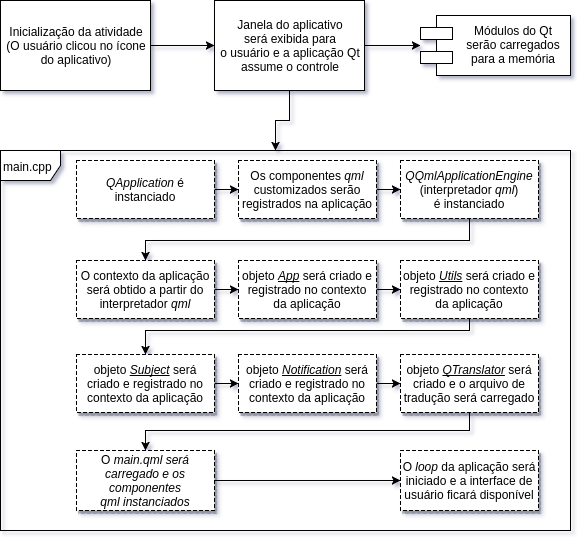
\includegraphics[width=8cm]{diagrama_fluxo_execucao}
	\centering
	\caption{\textit{workflow} da execução de um aplicativo Qt}
\end{figure}


\subsection{Métodos para utilização da arquitetura}
% descrever o README do projeto no github
Para utilizar a arquitetura desenvolvida, é necessário seguir uma determinada ordem de atividades que serão descritas abaixo. O código fonte da arquitetura encontra-se em uma página do \textit{github}, no link \cite{codigo_fonte_url} e é necessário utilizar o \textit{git} para obter uma cópia e iniciar a criação de um aplicativo. É preciso configurar o ambiente de desenvolvimento Qt para android ou iOS, além de baixar o android \textit{SDK} e o \textit{NDK}. No primeiro \textit{build} do aplicativo (na versão para android), o \textit{Gradle} baixará algumas bibliotecas para a máquina do desenvolvedor requeridas para o funcionamento do \textit{push notification}. Para criar um aplicativo usando esta arquitetura basta seguir o passo-a-passo abaixo:\par

\begin{enumerate}
	\item Acessar a página do projeto no \textit{github} e criar um \textit{fork} para a conta do desenvolvedor.

	\item Em seguida, basta clonar o projeto para a computador que será utilizado. É possível também, clonar a partir da página do projeto e alterar a url de origem.

	\item Após finalizar o processo de clonagem via git, renomear a pasta clonada e o arquivo \textit{tcc.pro} para o nome do aplicativo a ser desenvolvido.

	\item Importar o projeto (arquivo .pro) no \textit{QtCreator} e configurar as plataformas suportadas pelo aplicativo.

	\item Abrir o arquivo \textit{config.json} presente na raíz do projeto (manualmente usando algum editor) ou pelo \textit{QtCreator} na aba Resources \textit{config.qrc/config.json} e configurar as propriedades do aplicativo como foi descrito na seção 4.10. Os valores pré-definidos foram setados apenas como exemplo.

	\item Abrir o arquivo \textit{AndroidManifest.xml} no \textit{QtCreator} e renomear o \textit{package name}, de \textit{org.qtproject.example} para o nome do pacote do aplicativo a ser desenvolvido.

	\item Para utilizar \textit{push notification}, é necessário criar um projeto do \textit{Firebase} e adicionar o suporte a \textit{push notification}\footnote{https://console.firebase.google.com/project/novo-projeto-do-firebase/notification}. Em seguida, configurar as opções do projeto do \textit{Firebase} e no final do \textit{wizard} de configuração é necessário exportar o arquivo \textit{google-services.json} e salvar na pasta \textit{android} e IOS substituindo os arquivos existentes, também criados apenas como exemplo.

	\item No android, é necessário mais um passo para habilitar o \textit{push notification}. É preciso editar o arquivo \textit{android/build.gradle} e renomear o valor da propriedade \textit{defaultConfig.applicationId} (linha 71) para o \textit{package name} do aplicativo.

	\item Para customizar as cores do aplicativo no android (\textit{Action Bar}, \textit{Status Bar} e na janela do aplicativo), basta editar o arquivo \textit{android/res/values/colors.xml}. A cor definida em \textit{colorPrimary} será utilizada como cor de fundo no ícone de notificações via \textit{push} ou local.

	\item Em seguida, adicionar os ícones do aplicativo no diretório \textit{android/res/drawable-(*)dpi} e \textit{ios/icons}. O projeto vem com ícones nos tamanhos ideais (para android). No android, é possível utilizar alguma ferramenta\footnote{https://jgilfelt.github.io/AndroidAssetStudio/icons-launcher.html} online para gerar os ícones. No iOS, é recomendável utilizar a interface do \textit{XCode} para importar os ícones, que serão mapeados no arquivo xml \textit{Info.plist} que é equivalente ao \textit{AndroidManifest.xml}.

	\item Se algum plugin precisar exibir a logo ou o ícone do aplicativo, deve ser adicionado uma cópia de um ícone na pasta \textit{images} que está na raiz do projeto. Os ícones da pasta \textit{android} ou \textit{ios} não serão acessíveis por objetos da aplicação e o ícone nesta pasta será utilizado em modo desktop. Neste mesmo diretório, está a imagem \textit{drawer.jpg} utilizada no menu do layout em pilha (\textit{Drawer menu}), ela será carregada se a propriedade \textit{showDrawerImage} for \textit{true} no arquivo de configuração e pode ser substituída pelo programador. A imagem \textit{default\_user\_image.svg} será utilizada no perfil do usuário e também pode ser substituída por outra que combine com o design do aplicativo.

	\item Escreva os plugins. As funcionalidades do aplicativo deverão ser implementadas através de plugins. É possível iniciar o desenvolvimento de um plugin a partir dos exemplos fornecidos. Os plugins não serão mapeados em arquivo qrc sendo necessário criá-los manualmente, mantendo-os em uma pasta com o nome do plugin seguido de um arquivo \textit{config.json}, além de aquivos QML e imagens. Tudo que tiver na pasta do plugin será empacotado no APK ou IPA. Não é recomendável utilizar o \textit{wizard} de adição de arquivos do \textit{QtCreator}, pois ele adicionará os arquivos em \textit{qml.qrc}, que contém os componentes internos e reutilizáveis criando um acoplamento entre plugins e núcleo, violando um requisito não funcional desta arquitetura.
\end{enumerate}
	\section{Avaliação Experimental}\label{sec:avaliacao-experimental}

Esta seção existe apenas no TCC. Ela não deve existir no pré-projeto.

Aqui será apresentado a estudo de avaliação conduzido para valiar a solução desenvolvida.
	\section{Conclusão}\label{sec:conclusao}
%\begin{enumerate}
%	\item retomar o texto, como na introdução e no resumo
%	\item reapresentar os resultados, conclusões...
%\end{enumerate}
Aqui será apresentado as conclusões obtidos em todo o trabalho, sejam elas positivas ou negativas.


\subsection{Limitações Deste Trabalho}
A lista a seguir apresenta as limitações identificadas nesta arquitetura.

\begin{enumerate}
	\item Não há suporte a plugins escritos em C++: esse recurso seria importante, pois permitiria aos plugins delegar a lógica de negócio e operações de baixo nível a objetos C++, em vez de componentes qml como é atualmente. O problema é que as classes C++ devem ser conhecidas em tempo de compilação, pois em um projeto Qt as classes C++ devem estar mapeadas no arquivo \textit{.pro} gerando um acoplamento do núcleo da aplicação com os plugins;

	\item Instalação de plugins somente durante o \textit{build:}: a arquitetura não suporta a instalação de plugins dinamicamente. Esse recurso permitiria estender as \textit{features} do aplicativo sem precisar de um \textit{rebuild} e novo \textit{deploy};

	\item Suporte somente a um tipo de autenticação na API de rede: A arquitetura suporta apenas \textit{Basic Authentication} nas requisições HTTP e carece de outros tipos de autenticação suportados por \textit{web services} RESTful, tais como \textit{OAuth}, \textit{BEARER}, \textit{DIGEST Auth} entre outros;

	\item Atualização da arquitetura: Para criar um aplicativo utilizando esta arquitetura requer alteração em diversos arquivos e isso implica em obter as atualizações futuras da arquitetura, pois os arquivos modificados serão sobrescritos e o desenvolvedor terá que atualizá-los manualmente. Seria interessante que todas as alterações necessárias fossem feitas em arquivos separados e durante o \textit{build} fosse feito o merge. Em projetos android usando a versão mais recente do gradle, é possível fazer merge do arquivo \textit{AndroidManifest.xml} e o próprio arquivo \textit{build.gradle} que contém as APIs do \textit{Firebase} e outras propriedades de instalação e deploy no android.
\end{enumerate}


\subsection{Trabalhos Futuros}
Os itens abaixo, apresenta os possíveis incrementos futuros na arquitetura para facilitar ainda mais o desenvolvimento de plugins e melhorar a qualidade de um aplicativo baseado neste projeto.

\begin{enumerate}
	\item Adicionar os componentes reusáveis em um módulo estilo \textit{qmldir} para que o \textit{import} não seja feito através de uma string via \textit{qrc} e sim, via módulo similar ao \textit{import} do \textit{QtQuick};

	\item Adicionar o suporte a outros métodos na API de requisições HTTP tais como \textit{PUT}, \textit{OPTIONS}, \textit{DELETE} e \textit{HEAD};

	\item Atualizar a implementação de \textit{push notification} para a API em C++ do \textit{Firebase} que já está em versão estável. Isso irá simplificar a API de notificações via \textit{push} evitando ligações com objetos java via \textit{JNI};

	\item Melhorar o suporte ao iOS atualizando as bibliotecas do \textit{Firebase} para a versão mais recente, pois o \textit{xCode} exibe \textit{warnings} de que a versão da biblioteca utilizada possui APIs \textit{deprecated}, além de melhorar o suporte aos componentes visuais em telas retina declarando \textit{font-size} e dimensões baseadas no \textit{DPI} do dispositivo;

	\item Permitir que durante o desenvolvimento em modo Desktop, as alterações nos arquivos dos plugins sejam identificadas e carregadas a cada execução da aplicação, não exigindo o \textit{rebuild} do projeto, similar ao que acontece com os arquivos mapeados no \textit{qrc}. Atualmente, os plugins são copiados para o diretório do executável somente durante o \textit{build};

	\item Utilizar o \textit{Observer} como único mecanismo de comunicação entre objetos, descartando o uso do sinal \textit{eventNotify} da classe \textit{App}. O \textit{Observer} já está disponível na arquitetura mais não está sendo utilizado entre os componentes internos. As classes \textit{Subject} e \textit{Observer} em \textit{src/core} foram implementadas para oferecer um mecanismo de comunicação por eventos reduzindo o \textit{overhead} na aplicação notificando somente os objetos interessados no evento.
\end{enumerate}

	% to produce the bibliography for the citations in your paper.
	\bibliographystyle{abbrv}
	\bibliography{references}

\end{document}